% details-of-test-conditions.tex

\textcolor{red}{
	\chapter{Thermal Analysis}
}
%\textcolor{red}{XXX note: layers might be at different temps, tested temps may not be exceeded.}


The thermal protection of a hypersonic launch system is essential to its operation, and resisting the aerothermal loading produced during launch is one of the most significant challenges that must be overcome before airbreathing launch systems can become a reality. The modified SPARTAN launch system in this study uses nearly the same thermal protection that is used in previous SPARTAN studies, which has been assumed to be able to protect the SPARTAN throughout its launch trajectory\cite{Preller2018a}. However, no detailed thermal analysis of the SPARTAN has been carried out to date. This section aims to analyse the thermal protection system of the SPARTAN, in order to determine whether it is sufficient for operation to a first approximation. In this section, the heat flux over the trajectory is modelled at various locations on the SPARTAN and third stage, and integrated over the trajectory using 1-D heat conduction analysis to determine the efficacy of the thermal protection system. In addition, the design of the SPARTAN's TPS is investigated to provide an indication of the sensitivity of the temperatures produced during launch to critical TPS design parameters. 


%\textcolor{red}{XXX I dont know how to express why reynolds analogy is not valid.. is it just radiating shock layer effects? Then why would it be specific to a part of the leading edge that isnt near the shock?}


%For the body, the criteria for thermal protection system effectiveness is that the temperature at the internal surface of the thermal protection system does not cause failure in the internal structure. For the nose tips and the wing leading edges it is assumed that the thermal protection system will not be directly attached to the internal insulation and will have their own isolated structure, so that the criteria for thermal protection system success is that the temperature at these points is maintained within the operable limits of the external thermal protection system materials. 

\section{Heat Transfer Calculation}
The heat transfer coefficients on the body of the vehicle are computed using Reynolds analogy: 
\begin{equation}
c_h = \frac{c_f}{2s},
\end{equation}
where $c_f$ is the coefficient of friction and $s$ is the Reynold's analogy factor, assumed to be 1.16\cite{Ward2018}. 
This solution is performed within the viscous solver VC3D, at specific locations around the body of the scramjet accelerator and third stage, as shown in Figure \ref{fig:Q_pos}. On the scramjet accelerator, the nose stagnation point (\textcolor{red}{1}) and wing leading edges (\textcolor{red}{2}) are examined, along with a point midway along the nose (\textcolor{red}{3}), as well as midway along the cowl front (\textcolor{red}{4}), one-quarter of the length along the wing (\textcolor{red}{5}), and on the tip of the tail (\textcolor{red}{6}) on the windward side. On the third stage, the stagnation point on the nose (\textcolor{red}{1}) is examined, along with a point half way along the nose cone (\textcolor{red}{2}), and a point half way along the cylindrical cowl (\textcolor{red}{3}) on the windward side. These points are judged to be locations of potential high heat loads on the vehicles, and are examined as likely worst-case examples for thermal analysis. 

\begin{figure}[!ht]
	
\begin{subfigure}{.5\textwidth}
	\centering
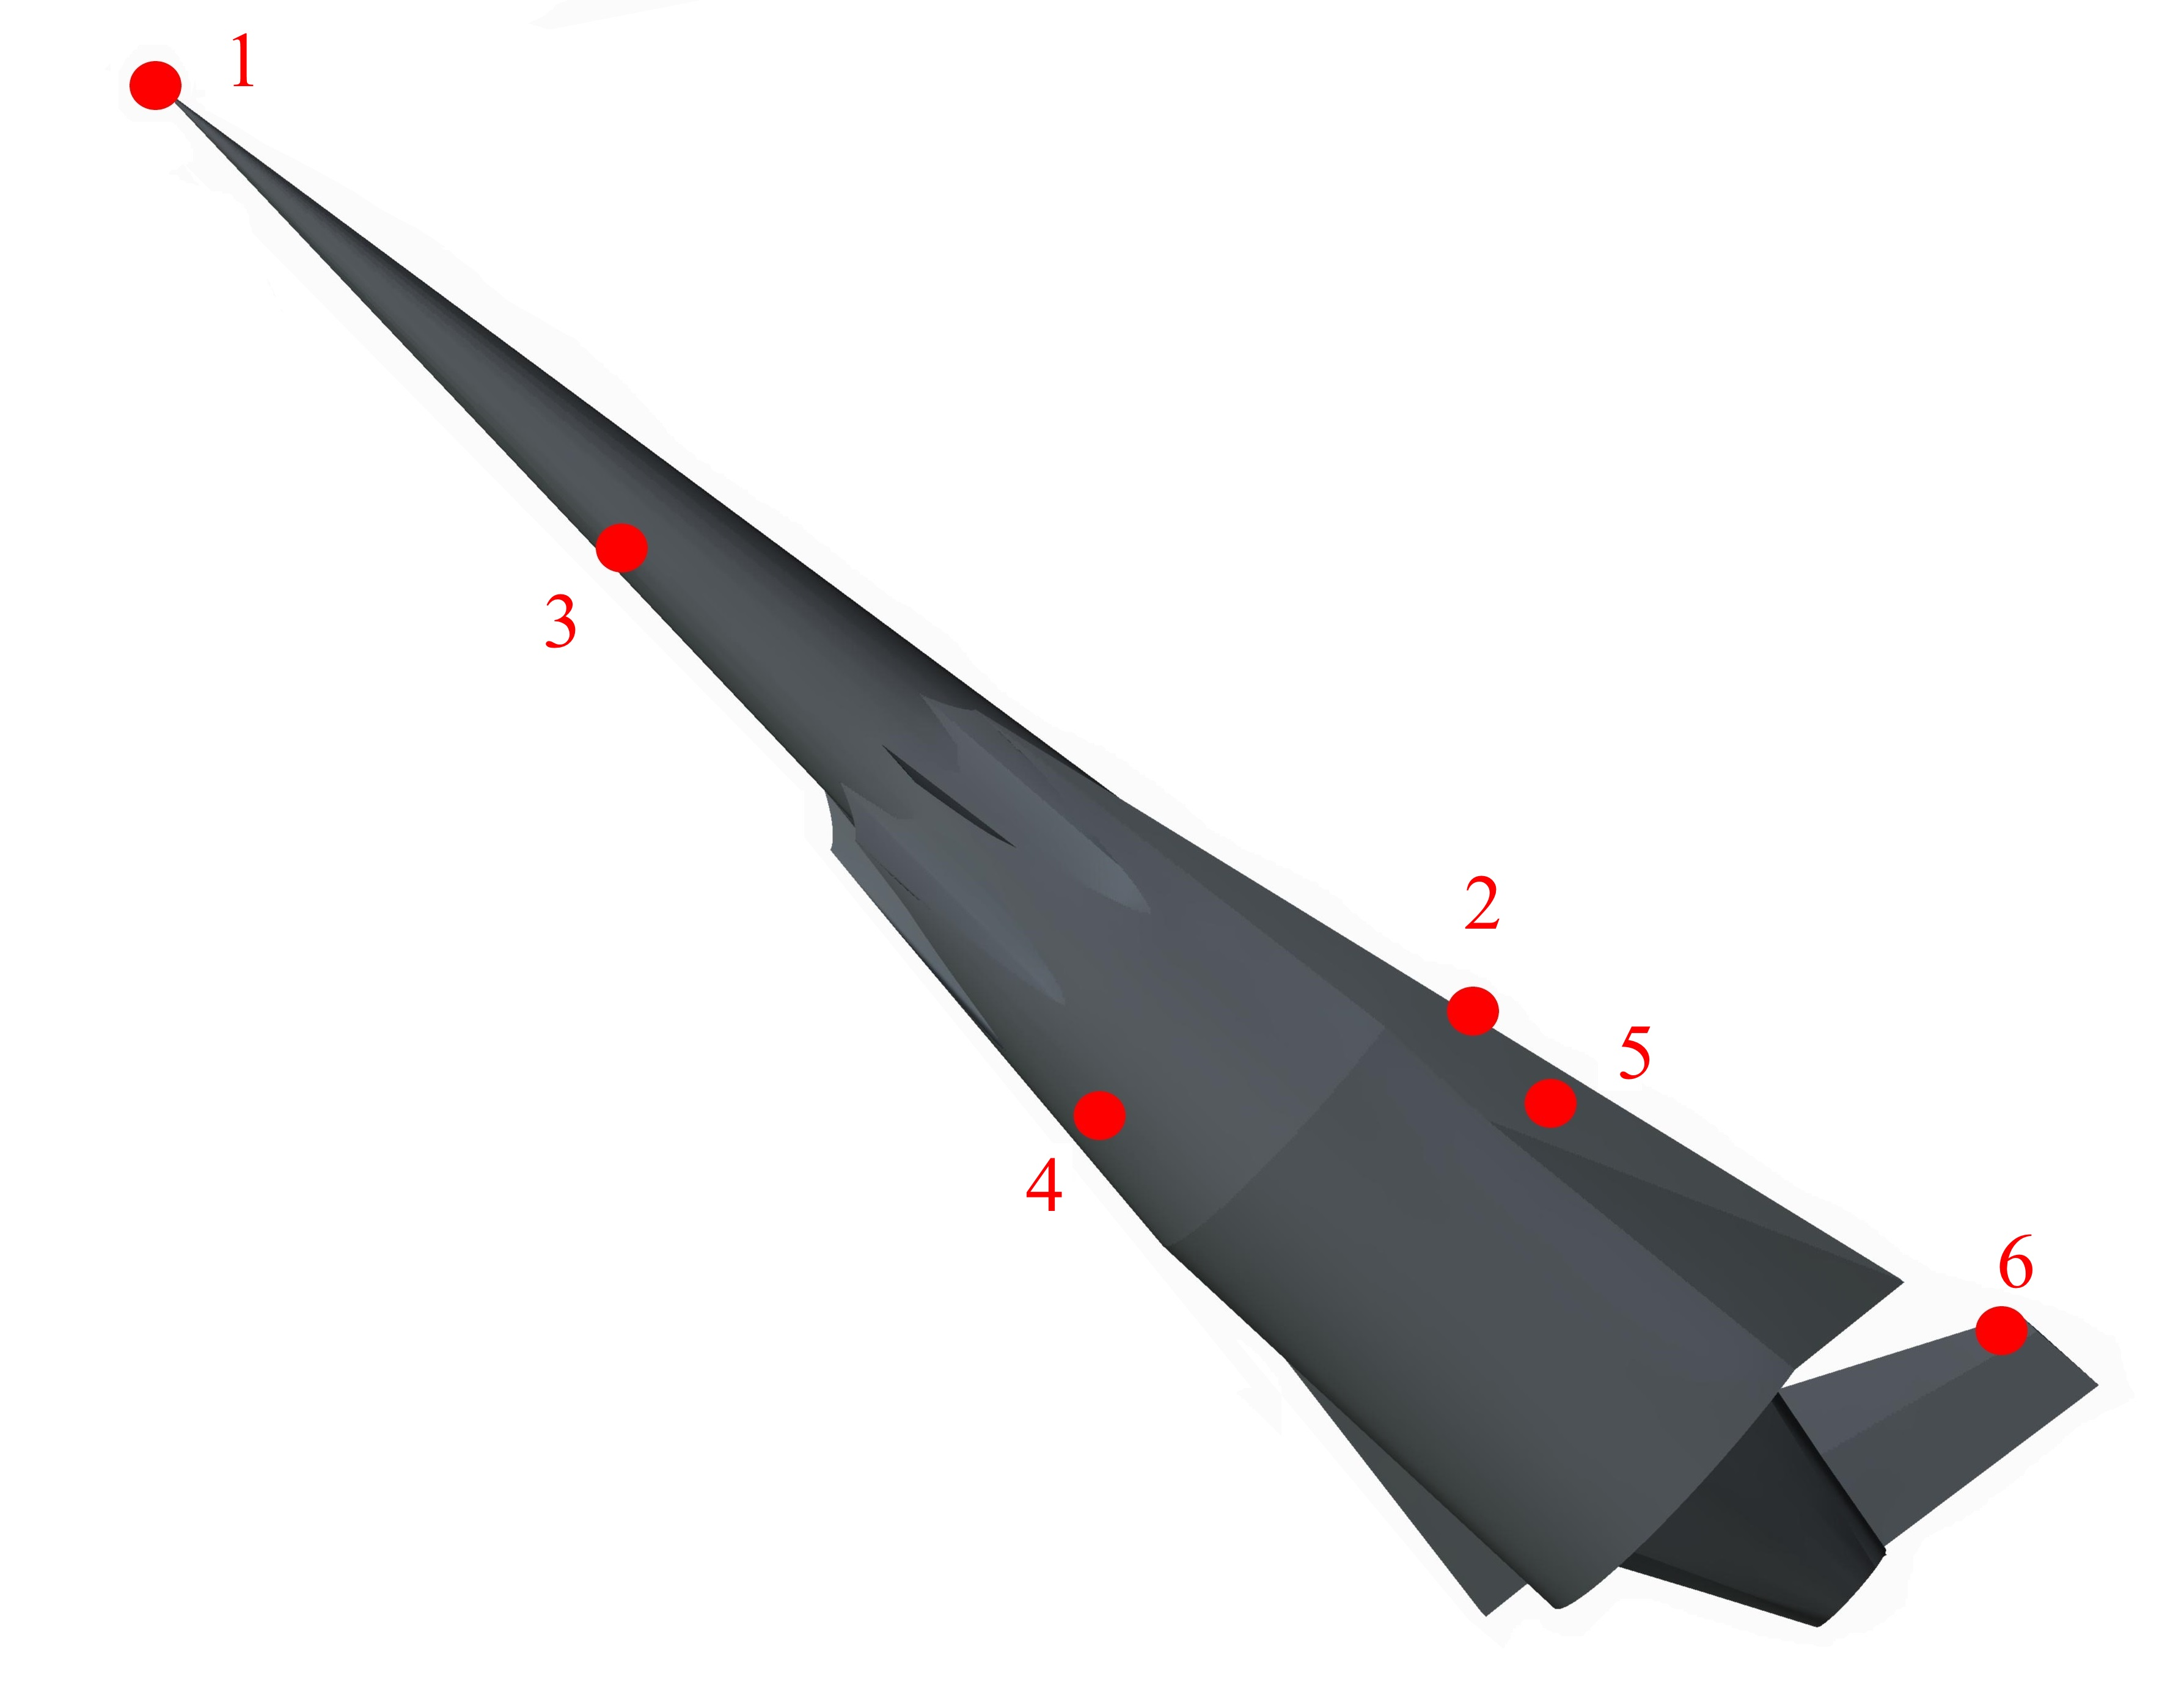
\includegraphics[width=0.9\linewidth]{figures/A1_uncertainty-analysis/Q_pos}
\caption{The points examined on the scramjet accelerator.}
\end{subfigure}
\begin{subfigure}{.5\textwidth}
	\centering
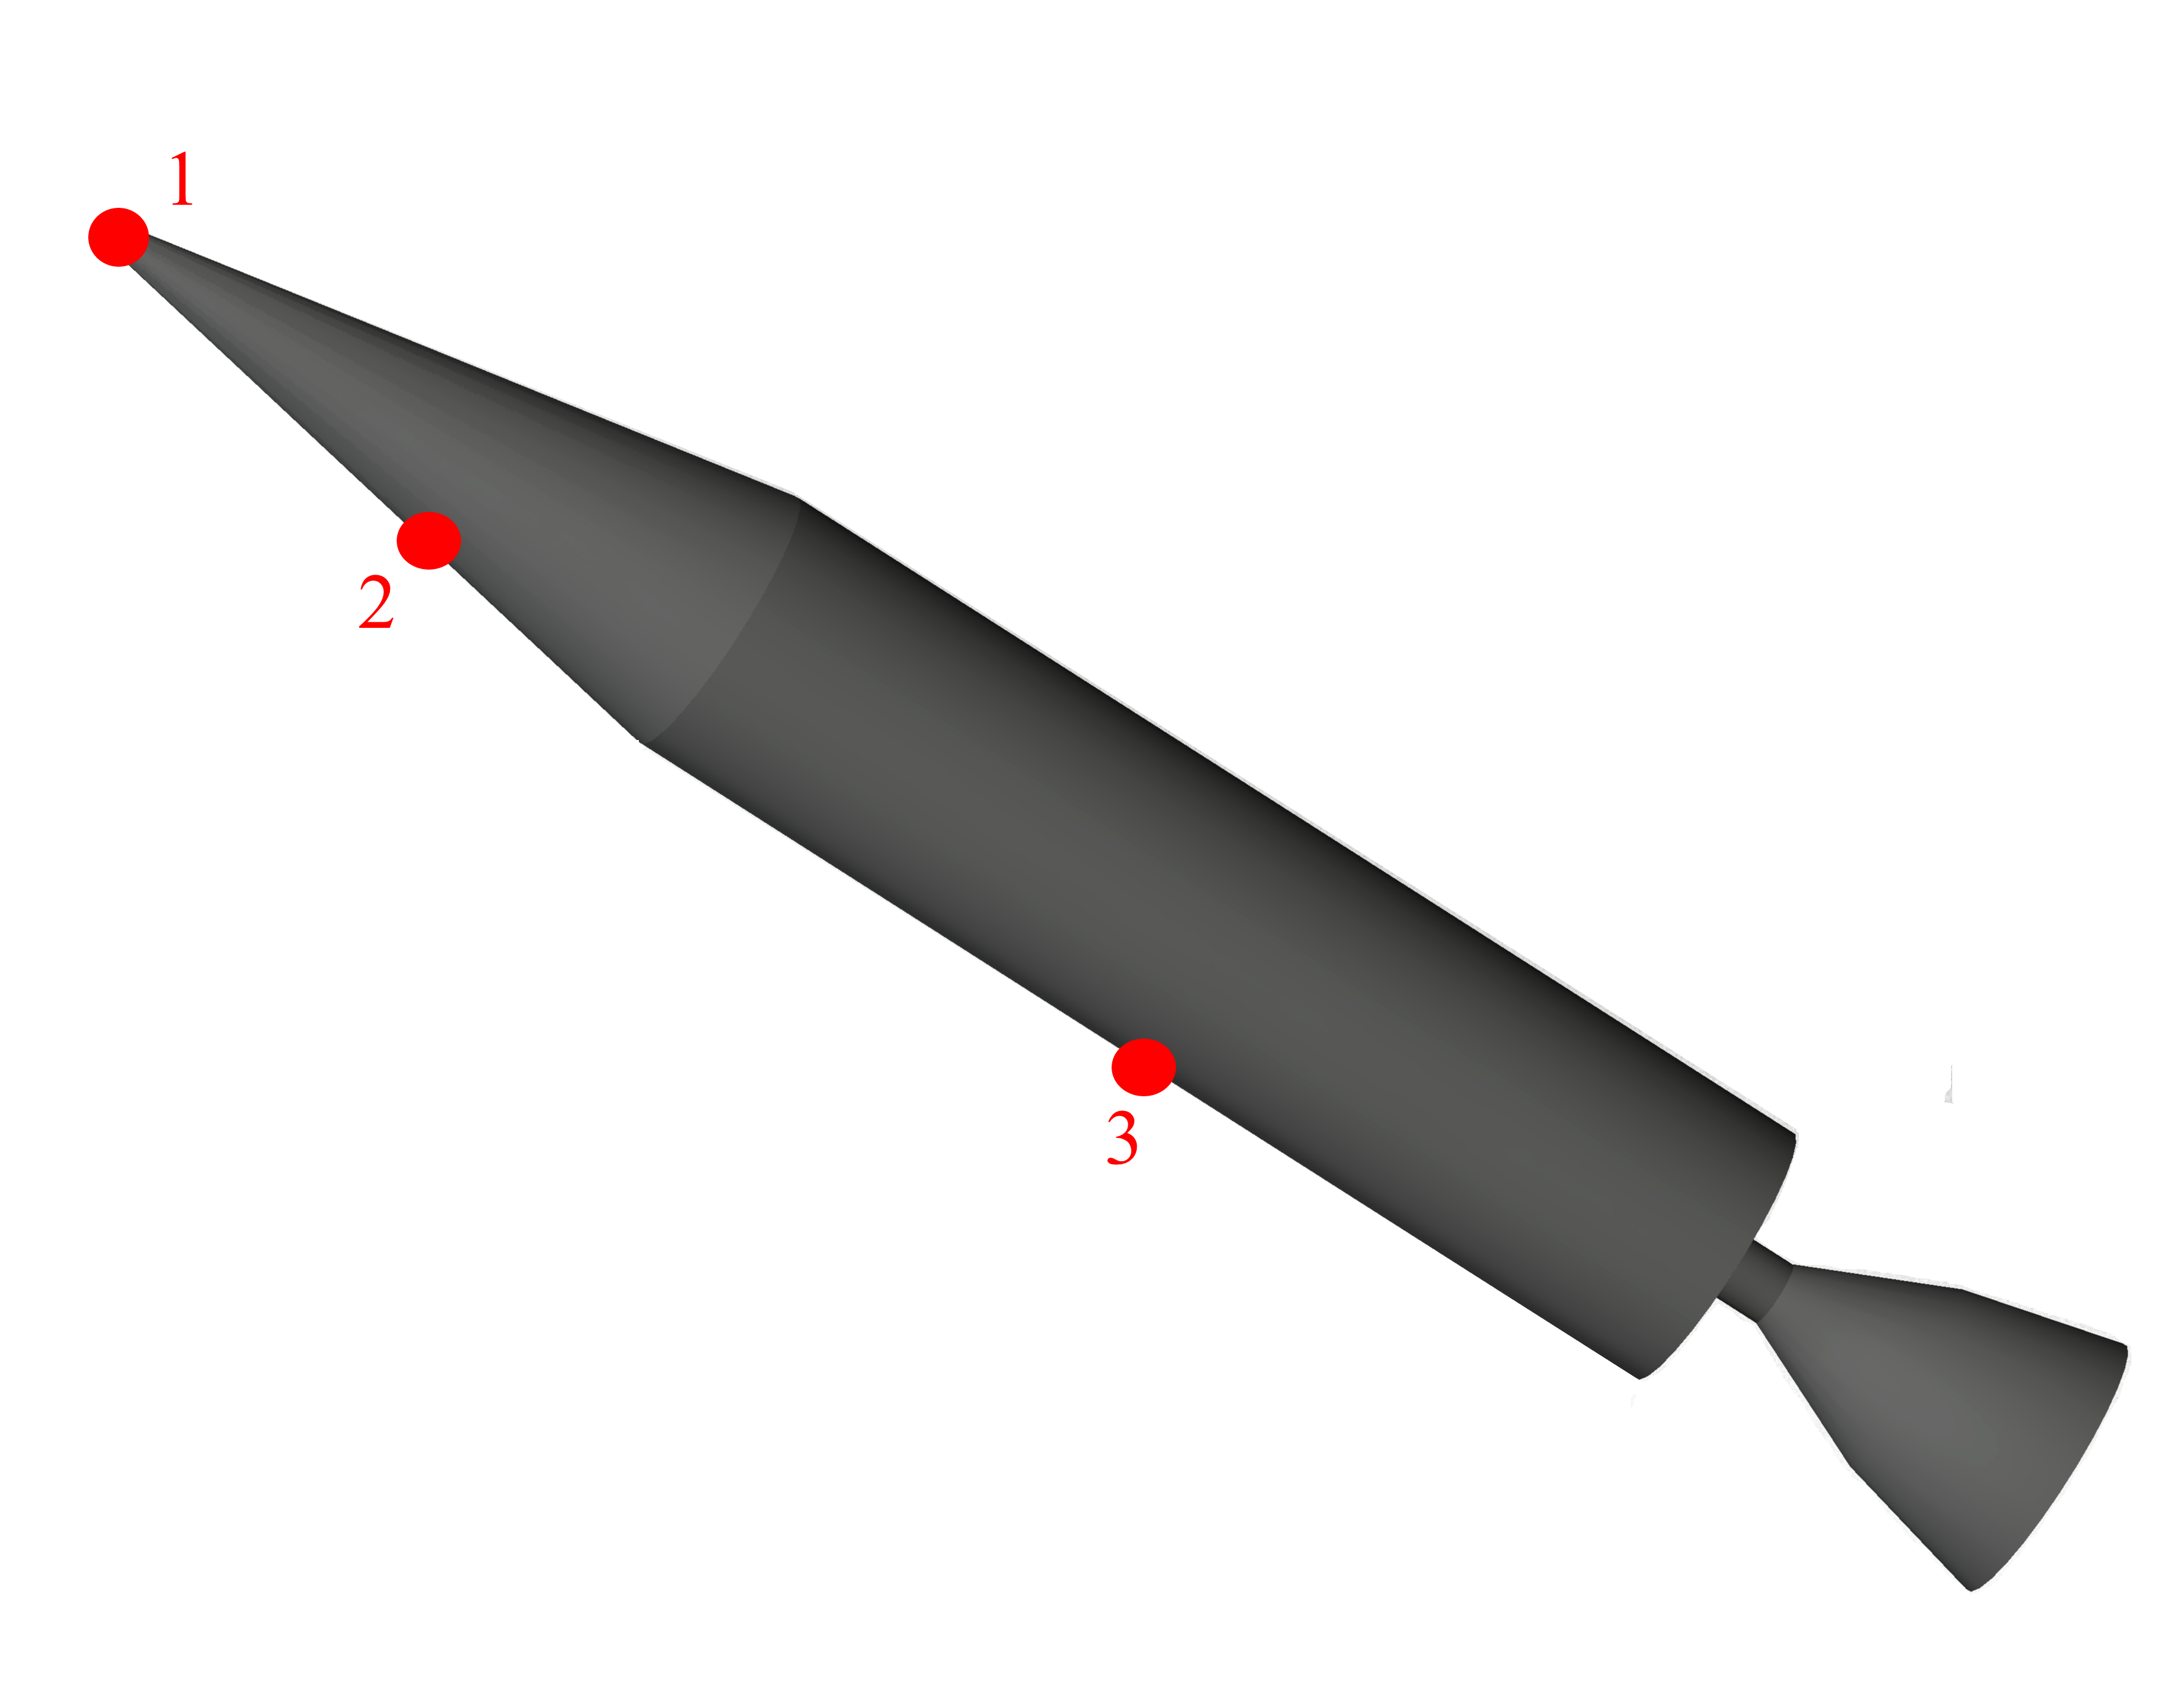
\includegraphics[width=0.9\linewidth]{figures/A1_uncertainty-analysis/Q_pos3}
\caption{The points examined on the third stage rocket.}
\end{subfigure}
\caption{The points chosen for thermal analysis, selected for the potential of high heat loading.}
\label{fig:Q_pos}
\end{figure}

The heat transfer at the stagnation point and leading edge of the wings, where Reynold's analogy is not valid due to large pressure gradients in the flow\cite{HypersonicGas}, is estimated using semi-empirical correlations\cite{Dirkx}. At the stagnation point, the heat transfer is given by\cite{Dirkx}:
\begin{equation}
q_s = k_1\rho^{N_1}V^{N_2},
\end{equation}
where $N_1 = 0.5$ and $N_2 = 3$, and the constant $k$ is\cite{Dirkx}:
\begin{equation}
k_1 = \frac{1.83 \times 10^{-4}}{\sqrt{R_n}}(1-\frac{T_w}{T_{aw}}),
\end{equation}
where $R_n$ is the nose radius, $T_w$ is the wall temperature, and $T_{aw}$ is the adiabatic wall temperature.

The heating at the leading edge is given by a weighted average correlation between a stagnation point and a flat plate\cite{Dirkx,Tauber2008}:
\begin{equation}
q_{LE} = (\frac{1}{2}q_s^2 \cos^2(\Lambda) + q_{FP}^2 \sin^2(\Lambda))^{1/2},
\end{equation}
where $\Lambda$ is the wing sweep angle, and the equation for a flat plate is calculated assuming turbulent flow under 2962m/s as:
\begin{equation}
q_{FP} = k_2\rho^{N_3}V^{N_4},
\end{equation}
where $N_3 = 3.37$, $N_4 = 0.8$ and
\begin{equation}
k_2 = 3.35 \times 10^{-4} \cos^{1.78}(\theta) \sin^{1.6}(\theta) x_T^{-1/5} (\frac{T_w}{556})^{-1/4} (1 - 1.11\frac{T_w}{T_{aw}}),
\end{equation}
where $\theta$ is the flow incidence angle and $x_T$ is the distance along the body from the transition point\cite{Dirkx,Tauber2008}. For the purposes of the leading edge heating the transition point is assumed to be half the distance along the nose cone, and the transitional boundary layer length is assumed to be equal to the preceding laminar flow distance. Along with this assumption, the aeroheating is calculated at the start of the wing, providing a worst case scenario for the heating rate on the leading edge. 



%\textcolor{red}{XXX Need to put in recognition for Alex \& Ingo for thermal stuff}


\section{Thermal Analysis of the Optimised Trajectory With Fly-Back}
 

\begin{figure}[!ht]
	\begin{subfigure}{.5\textwidth}
		\centering
		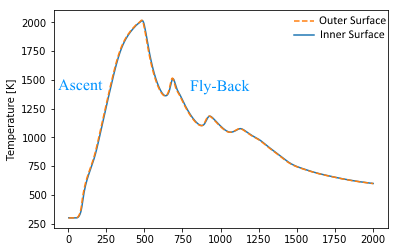
\includegraphics[width=0.99\linewidth]{figures/A1_uncertainty-analysis/TNoseReturn}
		\caption{The temperature time history at the nose (\textcolor{red}{1}.}
		
	\end{subfigure}
	\begin{subfigure}{.5\textwidth}
		\centering
		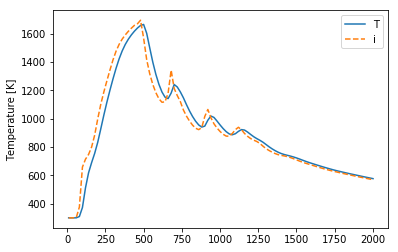
\includegraphics[width=0.99\linewidth]{figures/A1_uncertainty-analysis/TLEReturn}
		\caption{The temperature time history at the wing leading edge (\textcolor{red}{2}).}
		
	\end{subfigure}
	\begin{subfigure}{.5\textwidth}
		\centering
		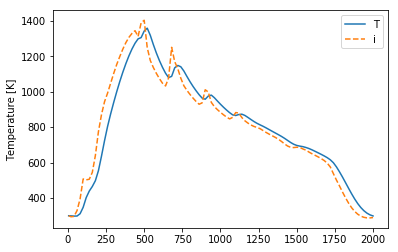
\includegraphics[width=0.99\linewidth]{figures/A1_uncertainty-analysis/TPos1Return}
		\caption{The temperature time history on the nose cone (\textcolor{red}{3}).}
		
	\end{subfigure}
	\begin{subfigure}{.5\textwidth}
		\centering
		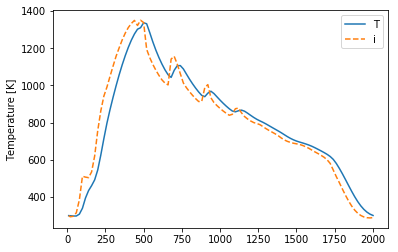
\includegraphics[width=0.99\linewidth]{figures/A1_uncertainty-analysis/TPos2Return}
		\caption{The temperature time history on the cowl (\textcolor{red}{4}).}
		
	\end{subfigure}
	\begin{subfigure}{.5\textwidth}
		\centering
		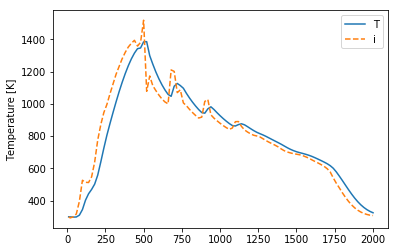
\includegraphics[width=0.99\linewidth]{figures/A1_uncertainty-analysis/TPos3Return}
		\caption{The temperature time history on the wing (\textcolor{red}{5}).}
		
	\end{subfigure}
	\begin{subfigure}{.5\textwidth}
		\centering
		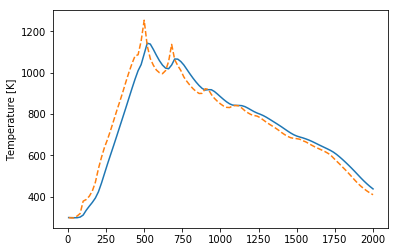
\includegraphics[width=0.99\linewidth]{figures/A1_uncertainty-analysis/TPos4Return}
		\caption{The temperature time history on the tail (\textcolor{red}{6}).}
		
	\end{subfigure}
	\caption{Temperature time histories on the scramjet accelerator.}
	\label{fig:TrajTemp}
\end{figure}


 
To determine the effectiveness of the SPARTAN's TPS system, a 1-D heat analysis is conducted.  
This heating calculation is implemented through the \textsf{uqTurbine} software package for 1-D heat transfer calculation, using the heat transfer calculations defined in the preceding section. 
This gives an indication of the temperature at the specified points around the SPARTAN throughout its trajectory. 
Figures \ref{fig:TrajTemp} and \ref{fig:TrajTemp3} show the heat responses at the specified locations on the vehicles over the ascent trajectory of the SPARTAN. 

The tungsten nose reaches 2015.1K, and the Carbon-Carbon wing leading edge reaches 1665.8K. 
At the nose and leading edge it is assumed that there is no direct thermal connection to the internal insulation by the structure or TPS at the regions of maximum heat loads. The maximum heating in this area is therefore assumed to be limited by the properties of the TPS itself. These temperatures are within the operational regimes of the external TPS materials, however, the TPS in these areas will need to be carefully designed to support the high structural loading of hypersonic flight, while also providing sufficient thermal isolation of the nose tip and leading edges.


\begin{figure}[!ht]
	\begin{subfigure}{.495\textwidth}
		\centering
		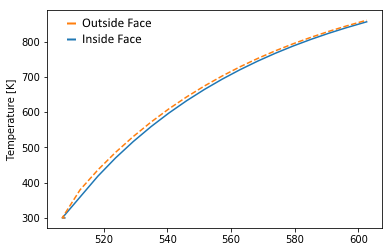
\includegraphics[width=0.99\linewidth]{figures/A1_uncertainty-analysis/TNose3}
		\caption{The temperature time history at the nose (\textcolor{red}{1}).}
		
	\end{subfigure}
	
	\begin{subfigure}{.495\textwidth}
		\centering
		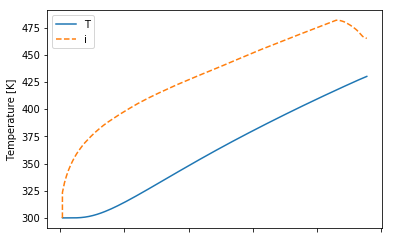
\includegraphics[width=0.99\linewidth]{figures/A1_uncertainty-analysis/T3onNose}
		\caption{The temperature time history on the nose cone (\textcolor{red}{2}).}
		
	\end{subfigure}
	
	\begin{subfigure}{.495\textwidth}
		\centering
		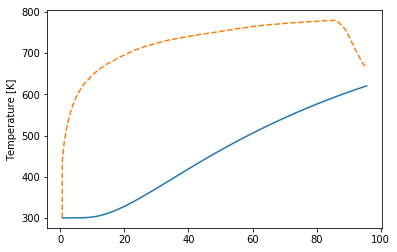
\includegraphics[width=0.99\linewidth]{figures/A1_uncertainty-analysis/T3Body}
		\caption{The temperature time history on the cylindrical body (\textcolor{red}{3}).}
		
	\end{subfigure}
	
	\caption{Temperature time histories on the third stage rocket with time.}
	\label{fig:TrajTemp3}
\end{figure}

On the body of the scramjet accelerator, the interior of the nose cone reaches a maximum of 1363.1K, the cowl 1384.9K, the wing 1326.4K, and the tail 1142.3K on the inner-face of the TPS.
These temperatures are well within the operational regime of the TPS material, although the internal temperatures are at the limits of the operational regime of the internal multilayer insulation, which is nominally designed for operation in the 900-1100$^\circ$C (1173-1373K) range. These high temperatures will begin to reduce the mechanical strength of the internal insulation\cite{Kourtides}, and must be accounted for in the detailed internal design, so that the internal insulation does not fail when peak temperatures are reached. Fibers with high strength at these high temperatures must be used in the internal insulation, and the aerodynamic loading must be distributed in such a way that the loads on the internl insulation do not cause mechanical failure. In this work it is assumed that the internal structure and insulation of the scramjet accelerator has been designed appropriately to account for regions of high heat load. For the purposes of this study, this is assumed to be sufficient for operation, however, detailed analysis of the TPS design, including analysis of the external TPS materials, as well as the internal multilayer insulation, must be conducted as the design of the TPS system of the SPARTAN is progressed. 

In addition to the high temperatures possibly approaching the limits of the multilayer insulation, the high temperatures produced will influence the material used for the internal structure. 
In analytical studies based on experimental tests of the internal multilayer insulation at 1273K (1000$^\circ$C) approximate surface temperature, the back face of the insulation has been shown to keep temperatures below 546K (273$^\circ$C)\cite{Kourtides} when the multilayer insulation with best performance (silica felt insulation\cite{Kourtides}) is used. Because the internal temperatures are above the experimentally tested temperature, the backface temperature of the insulation is likely to be above 546K, and are likely to be within the range where conventional aluminium alloys begin to lose their mechanical strength. Because of this, it is likely that a high temperature aluminium alloy would be required for the internal structure, at least in the regions of the internal structure that are close to the interface with the external insulation.

The temperatures on the third stage rocket are significantly lower than those experienced by the scramjet accelerator. The nose tip of the third stage reached a maximum inner face temperature of 874.8K, while the nose cone and body reach maximum temperatures of 439.4K and 655.8K respectively. These relatively low temperatures indicate that it may be possible to reduce the mass of the heat shield, by reducing the thickness of the tungsten and C-C protection on the nose, or by changing the material entirely. 


%Max temps: T0 T1

%nose:
%1945.4358   1947.8085 

%LE
%1665.796    1695.4998 

%on body:
%Pos 1 - 1361.0127  1435.0191
%Pos 2 - 1337.0232  1350.7068 
%pos 3 - 1384.9077  1517.4993 
%pos 4 - 1142.2337  1290.9281 


%third stage:
%nose tip: 874.80659 879.44989 

%Nose: 439.38044 472.50722 
%Body: 377.97737 397.55307 




\section{Aerothermal Exploration}

The design of the thermal protection systems of the vehicles within an airbreathing launch system is critical to the successful operation of the system. While this work assumes that the TPS is sufficient for operation, the scramjet accelerator stage is flying close to its thermal limits, while the heat loading on the third stage rocket is significantly lower. 
As the modelling of the launch system improves, its is likely that the TPS will be redesigned and heat shielding redistributed to optimise the weight of each vehicle while accounting for heating distribution. A 1D sensitivity study of the TPS design is conducted in this section, to allow for an initial estimation of the effects of variations in the passive TPS design, as well as the effects of active cooling inclusion. 

\subsection{Scramjet Accelerator TPS Design Exploration}

The thickness, density, thermal conductivity and specific heat of the C-C heat shield on the shroud are varied by $\pm$10\%, to measure the effect of the TPS properties and design at the region of highest heating with direct connection to the internal insulation. The maximum inner face temperature recorded is shown in Table \ref{tab:tpsscramjet}. These variations indicate an inner face temperature sensitivity of -2.7K/\% to variation in thickness, -1.9K/\% to variation in density, and 0.6 K/\% to variation in thermal conductivity when varied from the standard CCAT T-300 properties. 
The effects of a 10\% variation in any of these properties is not particularly large. This indicates that if the maximum inner face temperature is to be reduced in an area of high heating through modification of the heat shield, the heat shield design or properties in that area must be modified significantly to produce a significant effect. 


%XXX  density is the same as specific heat 
\begin{table}[ht]
	\centering
	\begin{tabular}{|c|c|c|c|c|c|}
		\hline  & -10\% & -5\% & Standard & +5\% & +10\% \\ 
		\hline Thickness & 1418.0 & 1401.4 & 1384.9  &   1375.6&   1363.6\\ 
		\hline Density & 1408.6 &  1396.3  & 1384.9 &  1378.0&  1369.9\\ 
		\hline Thermal Conductivity &  1380.4 & 1382.9 & 1384.9 &  1388.9& 1393.6\\ 
		\hline 
	\end{tabular}
	
	\caption{Inner face temperatures in K on the shroud of the scramjet accelerator with variations in TPS properties.}
	\label{tab:tpsscramjet}
	\end{table}

If passive TPS is not sufficient, active cooling may be introduced in areas of high heat loads. This active cooling can take many forms, such as regenerative, film, and transpiration cooling\cite{Zhu2018}, all of which are currently being actively studied for applications to hypersonic vehicles. For the most critical areas of high heating on the scramjet body, regenerative cooling is assumed to be the most practical method of active cooling, and the complex effects of this cooling are approximated as a set rate of heat transfer away from the inner face that directly reduces the temperature of the inner face of the TPS. Inner face temperatures on the shroud with heat transfer rates from 0 to 20kW away from the inner face are compared in Table \ref{tab:regenerativecooling}. The inner face temperature shows a sensitivity of -5.2 K/kW to a constant rate of heat transfer applied to the inner face. 


\begin{table}[ht]
	\centering
	\begin{tabular}{|c|c|c|c|c|c|}
		\hline Heat Transfer Rate & Standard (0kW) & 5kW & 10kW & 15kW & 20kW \\ 
		\hline Maximum T (K) & 1384.9 & 1359.3 & 1333.4 & 1307.4 & 1281.2 \\ 
		\hline
\end{tabular}	
\caption{Maximum inner face temperature with a constant rate of heat transfer away from the inner face of the shroud.}
\label{tab:regenerativecooling}	
\end{table}



\subsection{Heating limited Trajectory}

\begin{table}[ht]
	
	\centering
	\begin{tabular}{l c c c c c } 
		\hline \textbf{Trajectory Condition}	q$_2$Lim:
		& Standard
		& 1700kW
		& 1600kW
		& 1500kW
		& 1400kW
		\\
		\hline \textbf{Payload to Orbit (kg)}
		& \textbf{\PayloadToOrbitheatLimStandard}
		& \textbf{\PayloadToOrbitheatLimSeventeenHundred}
		& \textbf{\PayloadToOrbitheatLimSixteenHundred}
		& \textbf{\PayloadToOrbitheatLimFifteenHundred}
		& \textbf{\PayloadToOrbitheatLimFourteenHundred}
		\\
		\textbf{Payload Variation (\%)}
		& \PayloadVarheatLimStandard
		& \PayloadVarheatLimSeventeenHundred
		& \PayloadVarheatLimSixteenHundred
		& \PayloadVarheatLimFifteenHundred
		& \PayloadVarheatLimFourteenHundred
		\\
		\textbf{Total $\eta_{exergy}$ (\%)}
		& \textbf{\totalExergyEffheatLimStandard}
		& \textbf{\totalExergyEffheatLimSeventeenHundred}
		& \textbf{\totalExergyEffheatLimSixteenHundred}
		& \textbf{\totalExergyEffheatLimFifteenHundred}
		& \textbf{\totalExergyEffheatLimFourteenHundred}
		\\
		\hline 
		\textbf{1$^{st}$ Stage $\eta_{exergy}$ (\%)}
		& \textbf{\firstExergyEffheatLimStandard}
		& \textbf{\firstExergyEffheatLimSeventeenHundred}
		& \textbf{\firstExergyEffheatLimSixteenHundred}
		& \textbf{\firstExergyEffheatLimFifteenHundred}
		& \textbf{\firstExergyEffheatLimFourteenHundred}
		\\
		\textbf{Separation Alt, 1$\rightarrow$2 (km)}
		& \firstsecondSeparationAltheatLimStandard
		& \firstsecondSeparationAltheatLimSeventeenHundred
		& \firstsecondSeparationAltheatLimSixteenHundred
		& \firstsecondSeparationAltheatLimFifteenHundred
		& \firstsecondSeparationAltheatLimFourteenHundred
		\\
		\textbf{Separation v, 1$\rightarrow$2 (m/s)}
		& \firstsecondSeparationvheatLimStandard
		& \firstsecondSeparationvheatLimSeventeenHundred
		& \firstsecondSeparationvheatLimSixteenHundred
		& \firstsecondSeparationvheatLimFifteenHundred
		& \firstsecondSeparationvheatLimFourteenHundred
		\\
		\textbf{Separation $\gamma$, 1$\rightarrow$2 (deg)}
		& \firstsecondSeparationgammaheatLimStandard
		& \firstsecondSeparationgammaheatLimSeventeenHundred
		& \firstsecondSeparationgammaheatLimSixteenHundred
		& \firstsecondSeparationgammaheatLimFifteenHundred
		& \firstsecondSeparationgammaheatLimFourteenHundred
		\\
		\hline 
		\textbf{2$^{nd}$ Stage $\eta_{exergy}$ (\%)}
		& \textbf{\secondExergyEffheatLimStandard}
		& \textbf{\secondExergyEffheatLimSeventeenHundred}
		& \textbf{\secondExergyEffheatLimSixteenHundred}
		& \textbf{\secondExergyEffheatLimFifteenHundred}
		& \textbf{\secondExergyEffheatLimFourteenHundred}
		\\
		\textbf{Separation Alt, 2$\rightarrow$3 (km)}
		& \secondthirdSeparationAltheatLimStandard
		& \secondthirdSeparationAltheatLimSeventeenHundred
		& \secondthirdSeparationAltheatLimSixteenHundred
		& \secondthirdSeparationAltheatLimFifteenHundred
		& \secondthirdSeparationAltheatLimFourteenHundred
		\\
		\textbf{Separation $v$, 2$\rightarrow$3 (m/s)}
		& \secondthirdSeparationvheatLimStandard
		& \secondthirdSeparationvheatLimSeventeenHundred
		& \secondthirdSeparationvheatLimSixteenHundred
		& \secondthirdSeparationvheatLimFifteenHundred
		& \secondthirdSeparationvheatLimFourteenHundred
		\\
		\textbf{Separation $\gamma$, 2$\rightarrow$3 (deg)}
		& \secondthirdSeparationgammaheatLimStandard
		& \secondthirdSeparationgammaheatLimSeventeenHundred
		& \secondthirdSeparationgammaheatLimSixteenHundred
		& \secondthirdSeparationgammaheatLimFifteenHundred
		& \secondthirdSeparationgammaheatLimFourteenHundred
		\\
		\textbf{2$^{nd}$ Stage Flight Time (s)}
		& \secondFlightTimeheatLimStandard
		& \secondFlightTimeheatLimSeventeenHundred
		& \secondFlightTimeheatLimSixteenHundred
		& \secondFlightTimeheatLimFifteenHundred
		& \secondFlightTimeheatLimFourteenHundred
		\\
		\textbf{2$^{nd}$ Stage Distance Flown (km)}
		& \SecondDistheatLimStandard
		& \SecondDistheatLimSeventeenHundred
		& \SecondDistheatLimSixteenHundred
		& \SecondDistheatLimFifteenHundred
		& \SecondDistheatLimFourteenHundred
		\\
		\textbf{2$^{nd}$ Stage Return Fuel (kg)}
		& \returnFuelheatLimStandard
		& \returnFuelheatLimSeventeenHundred
		& \returnFuelheatLimSixteenHundred
		& \returnFuelheatLimFifteenHundred
		& \returnFuelheatLimFourteenHundred
		\\
		\textbf{2$^{nd}$ Stage Return Distance (km)}
		& \returnDistheatLimStandard
		& \returnDistheatLimSeventeenHundred
		& \returnDistheatLimSixteenHundred
		& \returnDistheatLimFifteenHundred
		& \returnDistheatLimFourteenHundred
		\\
		\hline 
		\textbf{3$^{rd}$ Stage $\eta_{exergy}$ (\%)}
		& \textbf{\thirddExergyEffheatLimStandard}
		& \textbf{\thirddExergyEffheatLimSeventeenHundred}
		& \textbf{\thirddExergyEffheatLimSixteenHundred}
		& \textbf{\thirddExergyEffheatLimFifteenHundred}
		& \textbf{\thirddExergyEffheatLimFourteenHundred}
		\\
		\textbf{3$^{rd}$ Stage $t$, $q >$ 5kpa (s)}
		& \thirdqOverFiveheatLimStandard
		& \thirdqOverFiveheatLimSeventeenHundred
		& \thirdqOverFiveheatLimSixteenHundred
		& \thirdqOverFiveheatLimFifteenHundred
		& \thirdqOverFiveheatLimFourteenHundred
		\\
		\textbf{3$^{rd}$ Stage Fuel Mass (kg)}
		& \thirdmFuelheatLimStandard
		& \thirdmFuelheatLimSeventeenHundred
		& \thirdmFuelheatLimSixteenHundred
		& \thirdmFuelheatLimFifteenHundred
		& \thirdmFuelheatLimFourteenHundred
		\\
		\hline 
	\end{tabular} 
	\caption{Scramjet stage stagnation point heating limited trajectories, optimised for maximum payload-to-orbit with stagnation point heating calculated using a cold wall approximation. }
	\label{tab:stagLim}
\end{table}

\begin{figure}[!ht]
\centering
\includegraphics[width=0.9\linewidth]{H:/github-home/LODESTAR-revisions/ArchivedResults/20191126T170823mode151/SecondStageComparison}
\caption{Comparison of scramjet accelerator trajectories with varying stagnation point heating limits.}
\label{fig:SecondStageheatlimComparison}
\end{figure}


The aerothermal effects on a launch vehicle may also be reduced by limiting the aeroheating of the vehicle during flight. However, performing a 1-D heat transfer analysis within a trajectory optimisation loop is prohibitively computationally expensive. 
As such, to investigate the effects of limiting the maximum aerothermal heating on the SPARTAN's scramjet accelerator in a computationally efficient manner, the stagnation point heat flux is calculated in-loop using a cold wall approximation ($T_W/T_{AW} \approx 0$). This calculation of the heat flux is conservative, however it is useful for applying limits to the heat loading for optimal trajectory investigation. Stagnation point heat flux limits of 1700, 1600, 1500 and 1400kW are applied, based on the maximum non-limited stagnation point heat flux calculated using a cold-wall approximation, of 1770kW. Optimised trajectories calculated with these heat flux limits applied to the scramjet accelerator stage are presented in Table \ref{tab:stagLim}, and the trajectories of the scramjet stages are shown in Figure \ref{fig:SecondStageheatlimComparison}. 

From Table \ref{tab:stagLim} and Figure \ref{fig:SecondStageheatlimComparison} it can be observed that limiting the stagnation point heat flux has a significant effect on the optimised trajectory. However, it is also evident that the effects of the 1700kW and 1600kW limits are small, compared to the effects of 1500kW and 1400kW limits. 
This sharp change in trajectory shapes is caused by a distinct cut-off point at which the scramjet stage is no longer able to perform the manoeuvres necessary to perform a pull-up. When stagnation point heat flux is limited to 1700 or 1600kW, the scramjet stage compensates by flying a slower, higher trajectory after release from the first stage rocket, reaching maximum dynamic pressure later, and performing a larger pull-up. This flight path limits the velocity of the scramjet stage and manoeuvres into a favourable position, while still performing a pull-up manoeuvre. In these cases, maximum heat flux is only reached at the start of the pull-up manoeuvre. However, when the stagnation point heating rate is limited to 1500kW or 1400kW, the trajectory changes significantly. For these limits, the beginning of the scramjet stage trajectory conforms with the non-limited optimal flight path, but the stagnation point heating limit causes the scramjet stage to leave maximum dynamic pressure and climb in the middle of the trajectory, reducing efficiency and manoeuvrability, and removing the ability of the scramjet accelerator stage to perform a pull-up manoeuvre. This cut-off point is primarily driven by the lower limit on the velocity of the scramjet accelerator during flight, which limits the start-of-trajectory manoeuvres performed to enable the pull-up in the 1700kW and 1600kW heating limited trajectories. 

Generally, these optimised trajectory results indicate that heating limits imposed on the trajectory of the scramjet accelerator vehicle result in the vehicle flying a significantly less efficient trajectory in order to reduce heat loads. For small heating limitations this may be suitable, however, in general, it would be preferable to design the vehicle so that it is able to fly close to an optimal payload-to-orbit flight path without heating limits. 



\subsection{Third Stage TPS Design Exploration}\label{sec:thirdstageheat}

\begin{table}[!ht]
	\centering
	\begin{tabular}{|c|c|c|c|c|c|}
		\hline Property & -10\% & -5\% & Standard & +5\% & +10\% \\ 
		\hline Thickness & 463.5 & 448.7 & 439.4 &  429.4 & 420.8  \\ 
		\hline Density &  456.5 & 447.5 & 439.4 & 432.0 &  425.2\\ 
		\hline Thermal Conductivity & 436.8 & 438.2 & 439.4 & 440.5 & 441.4 \\ 
		\hline 
	\end{tabular} 
	
	\caption{Inner face temperatures in K with variations in third stage TPS properties.}
	\label{tab:tpsthirdstage}
\end{table}

To explore the design of the third stage TPS, various properties of the C-C on the conical nose cone are varied by $\pm$10\%, and the temperature time histories along the optimised payload-to-orbit trajectory with return (Case 11) are calculated. The maximum temperatures observed on the inner face at the centreline of the nose cone TPS are shown in Table \ref{tab:tpsthirdstage}. These variations show an inner face temperature sensitivity of -2.1 K/\% to variation in thickness, -1.6 K/\% to variation in density, and 0.2 K/\% to variation in thermal conductivity when varied from the standard CCAT T-300 properties. These variations are relatively small, however, part of the reason for this is that the heat transfer, and the temperatures, are relatively low. 






\subsection{The Effects of a Pull-Up on the Third Stage Heat Shield Design}\label{sec:TPSredesign}


\begin{table}[!ht]
	\centering
	
	\begin{tabular}{l c } 
		\hline \textbf{Payload to Orbit (kg)}
		& \textbf{\PayloadToOrbitTPSreduced}
		\\
		\textbf{Total $\eta_{exergy}$ (\%)}
		& \textbf{\totalExergyEffTPSreduced}
		\\
		\hline 
		\textbf{1$^{st}$ Stage $\eta_{exergy}$ (\%)}
		& \textbf{\firstExergyEffTPSreduced}
		\\
		\textbf{Separation Alt, 1$\rightarrow$2 (km)}
		& \firstsecondSeparationAltTPSreduced
		\\
		\textbf{Separation v, 1$\rightarrow$2 (m/s)}
		& \firstsecondSeparationvTPSreduced
		\\
		\textbf{Separation $\gamma$, 1$\rightarrow$2 (deg)}
		& \firstsecondSeparationgammaTPSreduced
		\\
		\hline 
		\textbf{2$^{nd}$ Stage $\eta_{exergy}$ (\%)}
		& \textbf{\secondExergyEffTPSreduced}
		\\
		\textbf{Separation Alt, 2$\rightarrow$3 (km)}
		& \secondthirdSeparationAltTPSreduced
		\\
		\textbf{Separation $v$, 2$\rightarrow$3 (m/s)}
		& \secondthirdSeparationvTPSreduced
		\\
		\textbf{Separation $\gamma$, 2$\rightarrow$3 (deg)}
		& \secondthirdSeparationgammaTPSreduced
		\\
		\textbf{2$^{nd}$ Stage Flight Time (s)}
		& \secondFlightTimeTPSreduced
		\\
		\textbf{2$^{nd}$ Stage Distance Flown (km)}
		& \SecondDistTPSreduced
		\\
		\textbf{2$^{nd}$ Stage Return Fuel (kg)}
		& \returnFuelTPSreduced
		\\
		\textbf{2$^{nd}$ Stage Return Distance (km)}
		& \returnDistTPSreduced
		\\
		\hline 
		\textbf{3$^{rd}$ Stage $\eta_{exergy}$ (\%)}
		& \textbf{\thirddExergyEffTPSreduced}
		\\
		\textbf{3$^{rd}$ Stage $t$, $q >$ 5kpa (s)}
		& \thirdqOverFiveTPSreduced
		\\
		\textbf{3$^{rd}$ Stage Fuel Mass (kg)}
		& \thirdmFuelTPSreduced
		\\
		\hline 
	\end{tabular} 
	\caption{Summary of a payload-to-orbit optimised trajectory with a 42.4kg third stage heat shield.}
	\label{tab:heatshieldreduced}
	
\end{table}

A pull-up at the end of the scramjet stage acceleration has been shown in Section XXX to be an integral part of the payload optimal trajectory for a rocket-scramjet-rocket launch system. This pull-up also has significant aerothermal benefits for the third stage rocket. When separated from a scramjet stage constrained to constant dynamic pressure, the third stage rocket exhibits temperatures of 2163.5K on the nose tip, 1336.6k on the nose cone, and 1047.8k on the body, much larger than the temperatures generated by a third stage separated after a pull-up manoeuvre, of 874.8k on the nose tip, 439.4k on the nose cone, and 655.8k on the body. It is likely that the temperatures generated after release from a constant dynamic pressure trajectory would be at the limits of the multilayer insulation, however when released after a pull-up, the temperatures are much lower. While it is desirable to have lower temperatures on the third stage, and lower temperatures may be required for payload survivability, it may also be desirable to redesign the TPS of the third stage specifically to take into account the conditions after release from a scramjet stage flying a pull-up. 

To illustrate the effects of redesigning the TPS of the third stage rocket, the third stage heat shield thickness is reduced. The effects of the pull-up on the heat shield temperatures are too large to apply the linear sensitivity relationship developed in Section \ref{sec:thirdstageheat}, so the thicknesses of the nose tip, nose cone and cylindrical body are all reduced proportionally to the percentage reduction in temperature when the third stage is released after a pull-up, when compared to a third stage released without a pull-up as shown in Section XXX. This resulted in a heat shield weighing 49.1kg. An optimised trajectory was produced using this heat shield mass, with results summarised in Table \ref{tab:heatshieldreduced}. The payload-to-orbit increases to \PayloadToOrbitTPSreduced, an increase of 15.4kg (11.7\%) when compared to an optimised trajectory with the full heat shield mass, and an increase of 75.5kg (204.9\%) when compared to a trajectory with the scramjet stage constrained to fly at constant dynamic pressure. 

%-const q with fly-back
%
%compare max temps to pull-up
%
%recuce heat shield thickness by amount corresponding to indicated trend in previous section
%
%re-do optimised trajectory with new heat shield mass
%
%
%nose tip:
%874 - pull-up
%
%2163.4634 - constq
%
%40\%
%
%nosecone:
%439 - pull-up
%
%1336.6335 - const q
%
%32.8\%
%
%body:
%
%377 - pull-up
%
%1047.8395 - constq
%
%36\%
%
%
%modified heat shield weight: 42.4kg
%
%simulation with reduced heat shield: 149.3kg to orbit


\section{Summary}

A 1-D heat conduction analysis has been conducted to investigate the aerothermal effects of flying a payload-to-orbit optimised trajectory on the SPARTAN launch system. Various points around the scramjet stage and third stage were investigated, either using stagnation point heat transfer correlations for the nose and leading edges, or Stanton numbers computed using Reynold's analogy for points on the body. It was found that the temperatures on the nose and leading edges of the scramjet stage were very large, at 1947K and 1695K respectively. On the body of the scramjet accelerator, the interior of the nose cone was found to reach a maximum of 1363K, the cowl 1337K, the wing 1384K, and the tail 1142K on the inner face of the TPS. These temperatures are close to the limits of the multilayer internal insulation, and will produce temperatures on the inside face of the multilayer insulation that will require a high temperature aluminium alloy to withstand. It may be necessary to introduce further methods of mitigating this heating in future designs of the SPARTAN or other airbreathing launch vehicles. To investigate possible mitigation strategies, key properties of the TPS of the scramjet-powered stage were varied by $\pm$10\% indicate an inner face temperature sensitivity of -2.7K/\% to variation in thickness, -1.9K/\% to variation in density, and 0.6 K/\% to variation in thermal conductivity 
Next, active cooling was approximated by a constant rate of heat transfer away from the inner face, exhibiting a sensitivity of -5.2 K/kW. Lastly, heating limitations were imposed on the optimal trajectory, which had only a small effect at limits of 1700 and 1600kW, requiring manoeuvring of the scramjet accelerator at the beginning of the trajectory. However, heating rate limitats of 1500 and 1400kW produced a distinct cutoff point at which the scramjet accelerator could no longer manoeuvre sufficiently at the beginning of the trajectory, so that the trajectory shape followed closely to the dynamic pressure and heating limits, and the performance of the launch system degraded significantly. 


The maximum temperatures of the third stage rocket were determined to be much lower, with the nose tip of the third stage reaching a maximum inner face temperature of 874K, the nose cone  439K, and the body 377K on the inner face of the TPS. These relatively low temperatures indicate that it may be possible to reduce the thickness of the heat shield, or change material properties if so desired. A sensitivity study was conducted on key TPS design parameters on the nose cone section of the heat shield, and it was found that the third stage has a nose cone inner face temperature sensitivity of -2.1 K/\% to variations in thickness, -1.6 K/\% to variations in density, and 0.2 K/\% to variations in thermal conductivity when varied $\pm$10\% from the standard CCAT T-300 properties. To illustrate the possible design implications of a pull-up manoeuvre, the third stage heat shielding was reduced in thickness proportionally to the reduction in temperature on each segment caused by a pull-up manoeuvre, resulting in a heat shield weighing 49.1kg. A trajectory optimised for payload-to-orbit with this heat shield mass increased in payload mass to \PayloadToOrbitTPSreduced kg, a 15.4kg (11.7\%) increase over a trajectory optimised with the standard heat shield mass, and an improvement of 75.5kg (204.9\%) over a constant dynamic pressure trajectory. 

These results provide a preliminary analysis of the TPS of the SPARTAN. Initial results indicate that the TPS may be assumed to be sufficient for operation, however, more detailed analysis and design is necessary. A thorough design study is necessary to determine the efficacy of a passive TPS, along with a design optimisation taking into account the trade-offs between the heat shielding, the internal multilayer insulation, and internal structure. 


\textcolor{red}{
\chapter{Modelling Uncertainties}
}

%-need to take into account that the error magnitudes estimated are only relative error (as above)

%-take into account that the values qoted for abeynayake paper are mean, and that the max errors are higher

This thesis aims to provide new insight into the operability and feasibility of multi-stage launch systems incorporating an air-breathing stage.
No such launch systems currently exist, and several of the technologies necessary for the successful operation of their systems and subsystems are in the research stage of development.
This means that that reliable performance data is not available, and while every effort has been made to apply accurate vehicle and subsystem models, it is acknowledged that several are not designed in detail or validated, and others had to be simplified during the modelling process. 
These simplifications and uncertainties are separated into two distinct parts; the simplifications that arise during vehicle design, and the uncertainties that arise from the modelling of the launch system performance. 

The design uncertainties that arise from simplifications during the design process affect the vehicle's geometry, structure and internal layout, and mass and mass-distribution. In this work the design process is necessarily simplified, and it is assumed that by making appropriate design choices the nominal vehicle can be constructed (i.e. it is assumed that the designer can achieve the representative design by selecting appropriate materials and layouts), and that the nominal vehicle is capable of flying an appropriate launch trajectory. In this stage it is important for the designer to be aware of the sensitivities and trade-offs between design input parameters and performance. These design simplifications are described in more detail in Section XXX, and their effects are expressed by the parameter-by-parameter sensitivity study conducted in Sections XXX and XXX. These sensitivity studies provide insights into how the design factors of the launch system impact on the performance of the launch system and the shape of the optimised trajectory.

The uncertainties that arise during the modelling of the performance of the launch system introduce differences between the actual launch system and the ``as-designed" nominal launch system. 
As the designer has no direct control over these uncertainties (Which are both aleatory and epistemic), we need to rely on a-priori experience and a stochastic approach to quantify how the ultimate performance of the vehicle will be different to the ``as designed" simulations. The aim of this chapter is to apply a systematic approach to develop an understanding of how these uncertainties may affect the performance of the launch system. To consider this we first estimate the modelling uncertainties associated with the representative launch vehicle, and then conduct a reduced Monte-Carlo simulation (using Latin Hypercube sampling) to characterise how the modelling errors and simplifications affect the performance of an otherwise ``known" vehicle.




 







\section{Aerodynamic and Propulsion Simulation Uncertainties}


The purpose of this study is to determine the capabilities and performance of a multi-stage airbreathing launch system through the calculation and analysis of an optimal flight path. The calculation of an optimal flight path requires a large number of aerodynamic and propulsive simulations in order to cover the possible flight regimes of the launch system. In addition, the analysis of an optimal trajectory does not require high fidelity modelling techniques for useful information to be generated, because it is the general performance of the system that is of interest, rather than the specific performance of the design. Because of these factors, the launch system in this study is analysed using medium and low fidelity modelling techniques chosen for their fitness-for-purpose for optimal trajectory analysis, with an emphasis on computational efficiency as well as accuracy.
The uncertainties in the propulsive and aerodynamic properties of the launch system modelled in this work must be estimated, as there are no flight test or experimental results available for the representative launch system analysed in this study. In this section an estimate of the aerodynamic and propulsive uncertainties associated with the trajectory optimisations in this work is provided, and a Latin hypercube analysis is carried out to determine the variance in a sample trajectory optimisation and to assess the validity of the optimal trajectory results. 

\subsection{Aerodynamic Uncertainty}\label{sec:aerounc}

% XXX Check uncertainty vs error

%\textcolor{red}{XXX I need to make sure this isnt contradicting my lit review at all, and should repeat some of this in my lit review.}

The aerodynamic coefficients of the SPARTAN in this work are calculated using an inviscid Euler solver, Cart3D, with a flat plate correction for the viscous forces. This is a medium fidelity method, which brings with it a significant associated uncertainty in the aerodynamics of the vehicle, particularly at subsonic and transonic conditions. Although the aerodynamics of the vehicle in this work are not experimentally validated, studies have previously compared Cart3D with experimental data for a number of geometries at various flight conditions. These experimental comparisons are utilised to estimate the uncertainty arising in the aerodynamic coefficients due to the use of Cart3D. The first two of these comparison studies do not correct for viscous forces, and so underpredict drag in almost all cases in the supersonic and hypersonic regimes.



%- 'A Low Subsonic Study of the NASA N2A Hybrid Wing-Body Using an Inviscid Euler-Adjoint Solver' has error, but its too hard to estimate the values  from this.. . sagerman gives some specific pressure results, but only some. Dalle and Chan both have some comparisons, but without numbers.  

%\textcolor{red}{XXX be really careful here, the reviewer will know this paper inside out}
Abeynayake \& Agon assess two missile geometries; a conventional missile at transonic and supersonic speeds, and a non-conventional missile that has a cruise missile profile and includes small wings at subsonic speeds\cite{Abeynayake2013a}. The study by Abenayake and Agon estimates the magnitude of the uncertainty of Cart3D in a comparison to experimental results, although no viscous correction is included, and so the lack of a viscous component significantly affects the aerodynamic coefficients, particularly drag. The uncertainty magnitudes are estimated in relative error, normalised by the average value of data points between 0$^\circ$ and 10$^\circ$ angle of attack for drag, or the value at 10$^\circ$ angle of attack in the case of the lift and pitching moment coefficients\cite{Abeynayake2013a}. Because of this normalisation, and because experimental data is not shown\cite{Abeynayake2013a}, the mean error values reported are used in this study, and it is noted that these relative errors only give an indication of the accuracy of a specific tool\cite{Abeynayake2013a}. It is found that when compared to experimental results, Cart3D has a mean error in drag of 31.3\% for subsonic, 23.5\% for supersonic, and 18.0\% for transonic cases\cite{Abeynayake2013a} when compared to wind tunnel data for the non-conventional missile at angle of attack values between -10$^\circ$ and 10$^\circ$ in the subsonic regime, and the conventional missile at angles of attack of 0$^\circ$ to 10$^\circ$ in the transonic and supersonic regimes. The mean relative error in lift was found to be 16.5\% for subsonic, 1.3\% for supersonic, and 28.7\% for transonic cases\cite{Abeynayake2013a}, and the error in pitching moment 22.0\% for supersonic and 67.1\% for transonic cases, with no subsonic error given\cite{Abeynayake2013a}.
In this comparison study Cart3D was not able to match experimental trends closely in the subsonic and transonic regimes. Errors of up to 80.2\% in drag are observed in the subsonic regime for an unconventional missile geometry\cite{Abeynayake2013a}, although observing that the CFD++ result is much closer to the experimental result, it follows that the drag error in Cart3D likely diminishes significantly at angle of attack values between -5$^\circ$ and 5$^\circ$. In the supersonic regime, Cart3D appears to closely match the experimental lift and drag trends, with an underprediction in the magnitude of the drag forces due to the absence of viscous forces. 
Cart3D had poor results when computing pitching moment, although it was occasionally able to match the magnitude of the pitching moment well Cart3D was not able to match the experimental pitching moment trends for either vehicle\cite{Abeynayake2013a}. The work by Abeynayake \& Agon indicates that the uncertainties associated with Cart3D are significant, particularly at angle of attack values greater than 5 in the subsonic and transonic regimes, and that it does not estimate pitching moment trends well. However, a portion of the uncertainty magnitudes are associated with the inviscid nature of Cart3D, particularly in the drag forces in the supersonic and hypersonic regimes.

Kiris et al. compare between experimental data and CFD codes to assess their performance on the Ares V\cite{Kiris2011}. Cart3D is compared to the Overflow and USM3D RANS solvers, on a full scale Ares V model with conditions matching those expected during flight. In this comparison an axial force difference of maximum 10\% was found, present in the supersonic regime due to the inviscid nature of Cart3D\cite{Kiris2011}. Cart3D, USM3D and Overflow were then compared against three wind tunnel tests with scaled vehicles, each with slightly different shroud or base shapes. Only one vehicle configuration produced results good enough for comparison\cite{Kiris2011}, showing high Cart3D error in the subsonic and transonic regimes. Cart3D was reported to exhibit maximums of 33\% error in axial force and a 17\% error in normal force in the subsonic regimes, 20\% error in axial force and 21\% error in axial force in the transsonic regime, and 19\% error in axial force and 12\% error in normal force in the supersonic regime, when compared to experimental results. In the supersonic regime, the axial force underpredicts consistently, and much of the axial force error is likely due to a lack of viscous effects in Cart3D. 

A study by Ward et al.\cite{Ward2018} compares Cart3D results to experimental results for a blunt body at hypersonic speeds, a lifting body vehicle at subsonic and supersonic speeds, and a hypersonic accelerator test geometry at hypersonic speeds. Ward et al. provide a method for viscous correction of the Cart3D results, and also compare this with experimental results, focusing on the amount that drag error is able to be corrected. In this study Cart3d was found to predict trends in drag coefficients well for all tested cases both subsonic and supersonic, although with a consistent underprediction of 15-25\% in drag coefficient due to a lack of viscous effects\cite{Ward2018}. When corrected for viscous effects, the drag coefficient was found to agree closely with the experimental results at supersonic and hypersonic speeds, with error reducing to less than 10\% for the hypersonic accelerator test vehicle, and less than 11\% for the lifting body at supersonic speed\cite{Ward2018}. Drag error at high angles of attack at subsonic speeds was still found to be large, at 38\%, however, at angles of attack under 5$^\circ$ the error reduced significantly, matching the experimental results to within 16\%. 


The three studies investigated here are used to assign uncertainties to the aerodynamic coefficients computed by Cart3D. These uncertainties are separated by subsonic, transsonic and supersonic/hypersonic regimes, because it is evident that Cart3D shows significantly varied and uncorrelated errors in each regime. Generally, the maximum of the error values reported is used as an approximation of the upper uncertainty bound for a given coefficient and regime. 
  Note that while the values reported by Abeynayake \& Agon\cite{Abeynayake2013a} are non-dimensionalised relative accuracies, it is assumed here that the mean values reported indicate the accuracy of Cart3D. 
  
  In the subsonic and transsonic regimes Abenayake \& Agon and Kiris etl al. find that Cart3D is not capable of predicting the trends of the aerodynamic data well\cite{Abeynayake2013a,Kiris2011}, and as such the uncertainty values for coefficients in these regimes are set to the maximum error values observed within the operable regions across the investigated works, when data is available.
  The subsonic drag uncertainty is set as 33\%, and lift uncertainty is set to 17\%, matching the  maximum error observed by Kiris et al.\cite{Kiris2011} in the axial and normal forces in this regime. 
The pitching moment error in the subsonic regime is not stated in any of the works analysed, so the average relative error for all Cart3D coefficients at subsonic speeds reported by Abeynayake \& Agon\cite{Abeynayake2013a}, 23\%, is used.
The drag uncertainty in the transonic regime is set to 21\%, to match the axial force error reported by Kiris et al.\cite{Kiris2011}, and the lift and pitching moment uncertainties in this regime are set to 28.7\% and 67.1\% respectively, to match the mean relative error reported by Abenayake \& Agon\cite{Abeynayake2013a}. 
The lift coefficient uncertainty in the supersonic regime is set to 12\%, to match the error reported by Kiris et al.\cite{Kiris2011}, and the pitching moment uncertainty is set as 22.0\%, to match the mean relative error reported by Abeynayake \& Agon\cite{Abeynayake2013a}. 
In the supersonic regime the ability of Cart3D to predict drag trends improves, with the lack of viscous effects causing a consistent underprediction in axial force while still matching experimental trends when uncorrected\cite{Abeynayake2013a,Ward2018,Kiris2011}. The uncertainty in drag in the supersonic regime is set to 11\%, to match the maximum error observed after viscous correction by Ward et al.\cite{Ward2018}, due to the observations that that the consistent underpredictions observed by Abeynayake \& Agon\cite{Abeynayake2013a} and Kiris et al.\cite{Kiris2011} are primarily due to a lack of viscous effects. The Euclidean correction method outlined by A. Ward was utilised to correct the inviscid aerodynamic coefficients in this study, with viscous aerodynamics provided by A. Ward for this work, warranting the use of the error value for axial force reported after viscous correction in the supersonic/hypersonic regime. 
These uncertainty values are summarised in Table \ref{tab:AppendixUncertainty}, along with the uncertainties in the propulsion systems. 




%\subsubsection{Uncertainties Associated With Realistic Flight}

%The sources of variations between pre-flight predictions of hypersonic vehicles and actual flights are numerous, including modelling and experimental uncertainty, as well as on-the-day variations in the flight environment, vehicle and atmosphere. A study was carried out by Cobleigh\cite{X33} to develop an uncertainty model for the now discontinued X-33 SSTO demonstrator aircraft. The study by Cobleigh utilised comparisons of pre-flight aerodynamic estimates developed using either wind tunnel or computer modelling to flight test estimates for six lifting body aircraft, as well as the space shuttle, to estimate uncertainties in the aerodynamics of the X-33 from Mach 0.1 to 12. 
%-I have no way to convert the error from the coefficients to something useful. Also the lift coefficient errors that they have produced seem ridiculous compared to even their own aero coeffs in other papers? but they are saying its well predicted?




\subsection{Propulsion System Uncertainties}\label{sec:propunc}




\subsubsection{The Rocket Engines}
The propulsive properties of the rocket engines that power the first and third stages of the launch system are taken from the Falcon 1 Launch Vehicle Payload User's Guide\cite{Vehicle2008}, a document released by SpaceX that does not contain detailed information as to how the engine properties are calculated. It is assumed that the properties of the engines presented by SpaceX have been measured experimentally, and that the primary uncertainties associated with the rocket engine properties are experimental uncertainties. With no knowledge of the experimental facilities or processes used, it is necessary to estimate the experimental uncertainty through analysis of other experimental facilities, information that is generally sparse. Davidian, Diek and Chuang\cite{Davidian1987} assess the specific impulse uncertainty associated with high area ratio rocket tests at NASA Lewis Research centre, by propagating an "exhaustive" list of possible error sources. The test facility was found to be capable of measuring specific impulse to within 1.30\%, thrust to within 1.12\%, and mass flow rate to within 0.72\%. These propagated uncertainty values assumed that there was no bias errors, and that calibration had no error prior to testing. 
The uncertainty in the specific impulse of 1.30\% is used as the rocket engine performance uncertainty for the purposes of this study, assuming that the testing that has been carried out on the Merlin 1-C and Kestrel engines has the same error margins as the NASA Lewis Research Centre facilities. 

\subsubsection{The Scramjet Engine}
%Quasi-One-Dimensional Model of Hydrogen-Fueled Scramjet Combustors". These are the studies that the engine models were likely tuned off 

%Ingo says that I might need to ballpark a number, say 25\%, but that it could be much higher, even 50\% in his optinion. I will need to be very clear here. 

%\textcolor{red}{XXX check with michael about the experimental corrections, is there a reference for it?}
%-ask michaael if crest database has experiomental results- ingo thinks that 1D ANalysis is tuned using ground test data. In this case it doesnt make much sense to work out uncertainty from ground test data.
The C-REST engines are modelled in this work using a dataset developed using a combination of high-fidelity CFD, and quasi 1-D analysis, tuned using experimental results\cite{Jazra2010}. Estimating the error in this model in comparison to a realistic, flight capable scramjet is not feasible, due to the lack of flight test data or full-scale engine ground testing for scramjet engines in the public domain. For the purposes of this study a nominal uncertainty of 25\% is associated with the specific impulse of the scramjet engines based on the experience of the Author's colleagues and supervisors at The University of Queensland's Centre for Hypersonics. This is an estimated uncertainty margin, and it is possible that the uncertainty margin may be higher than this estimated value. However it is probable that if there is errors larger than 25\% in the performance modelling of the scramjet engines, then the design of the system may have to change considerably to be feasible. For this reason, the uncertainty margin of the scramjet specific impulse is kept at 25\% for payload-to-orbit uncertainty margin calculations, although it is acknowledged that major unforseen modelling or experimental errors may cause design changes to be necessary or lead to the infeasibility of the system as a whole. 


\subsection{Quantification of Aerodynamic and Propulsion Uncertainty Effects}


The uncertainty margins of the aerodynamic and propulsive data for the representative launch system analysed in this study are shown in Table \ref{tab:AppendixUncertainty}. These uncertainty margins have been developed in Sections \ref{sec:aerounc} \& \ref{sec:propunc}, based on studies comparing the modelling techniques used in this study to higher fidelity techniques and experimental data.  

%-note that it is assumed that only the moments on the SPARTAN are affected, and not the flaps

\begin{table}[ht]
	\centering
	\begin{tabular}{|c|c|c|c|}
		\hline  Uncertainty & Subsonic & Transonic  & Supersonic/Hypersonic \\ 
		\hline  1$^{st}$ \& 3$^{rd}$ Stage $I_{SP}$ & 1.3\% & 1.3\% &  1.3\% \\ 
		\hline  Scramjet $I_{SP}$ & - & - &  25\% \\ 
		\hline   $C_L$ & 17\% & 28.7\% & 12\% \\  
		\hline   $C_D$ & 33\% & 21\% & 11\% \\  
		\hline   $C_M$  & 23\% & 67.1\% &  22.0\% \\ 
		\hline 
	\end{tabular}
	\caption{The uncertainty margins associated with the aerodynamic and propulsive modelling of the SPARTAN. Values are shown to the accuracy measured or reported from their source.}
	\label{tab:AppendixUncertainty}
\end{table}



\begin{figure}[ht]
	\centering
	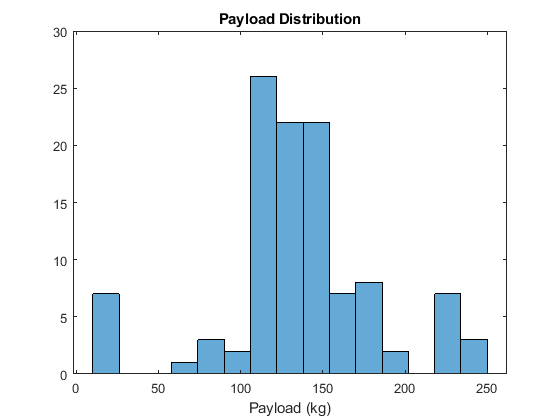
\includegraphics[width=0.7\linewidth]{figures/A1_uncertainty-analysis/LHC}
	\caption{The distribution of optimised payload-to-orbit values over the range of LHC determined samples.}
	\label{fig:LHC-17bins}
\end{figure}

In order to quantify the effects of the modelling uncertainty in the aerodynamic and propulsion models, a Monte Carlo variation study is carried out using a Latin Hypercube Sampling technique. A sample size of 100 runs was used, distributed using Matlab's \textsf{lhsdesign} function. This distribution is assumed to be normally distributed, producing a 2-$\sigma$ deviation of $\pm$106.9kg in payload-to-orbit. This deviation illustrates the large uncertainties still present in the modelling of airbreathing launch systems, however, this is to be expected for studied of launch systems that are still early in their conceptual design phases, particularly given the general sensitivity of the payload mass in launch systems to variations in the launch system performance. However, this interval also indicates that producing a positive payload-to-orbit is likely to be possible under the current modelling scheme, although it is evident that more detailed analysis of this system is necessary before an accurate payload-to-orbit value is able to be attained. This said, the payload-to-orbit values calculated in this study are only intended as an indication of the performance possible using this launch system, and are primarily utilised in comparison studies, to produce trends in performance that have been analysed in Chapters XXX and XXX. These performance trends are still valid and useful, even though they fall well within the uncertainty margins of the payload mass and performance of the launch system.




\section{Atmospheric Variations}
\subsection{Seasonal and Solar Cycle Based Variations}

\begin{figure}[ht]
	\centering
	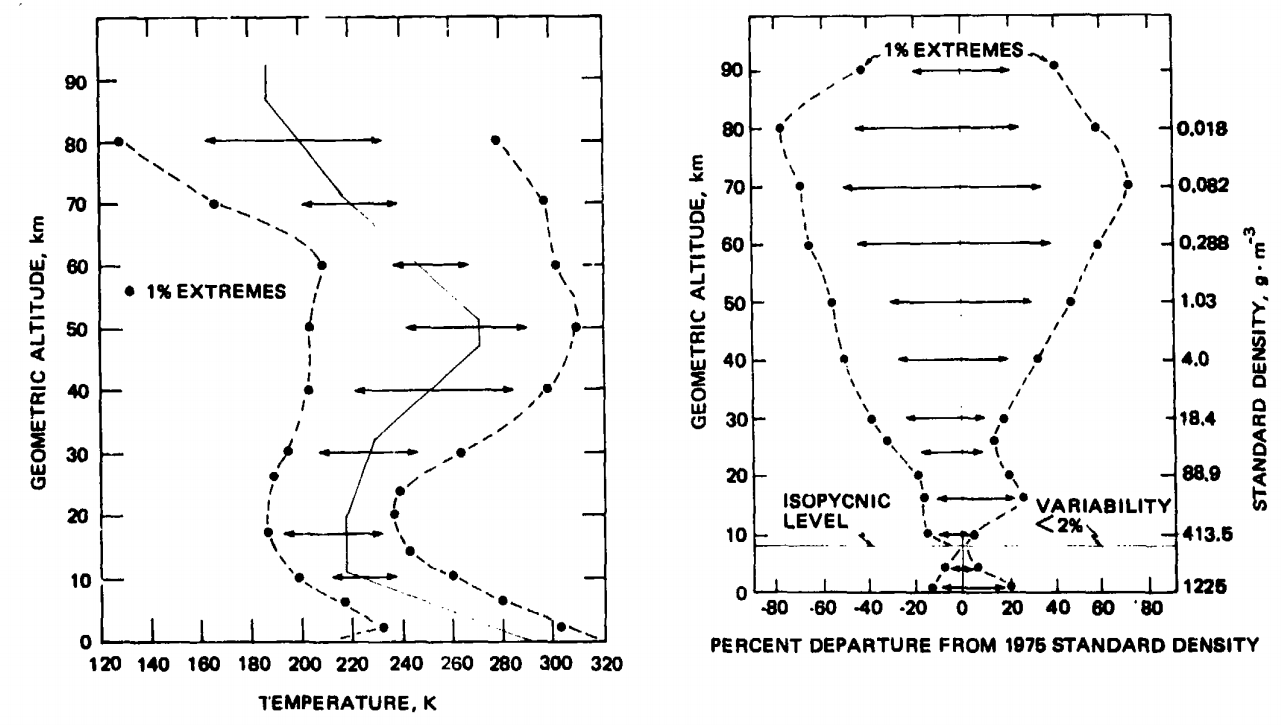
\includegraphics[width=0.8\linewidth]{figures/A1_uncertainty-analysis/AtmosphericVariation}
	\caption{Variation in temperature and density in the 1976 U.S Standard Atmosphere Model\cite{Administration1976}. Arrows indicate lowest and highest mean monthly values obtained at any location, and dashed lines indicate one-percent extremes.}
	\label{fig:AtmosphericVariation}
\end{figure}

The Earth's atmosphere varies significantly depending on location, and over time. Seasons, solar cycles, and general weather effects all contribute to these variations, which are numerous and difficult to predict. As such, the atmosphere into which the SPARTAN is launched may be considerably different to the atmosphere that is being modelled in this work. 
Atmospheric variations may affect the aerodynamic and engine performance of the launch system significantly, and change the altitude at which the maximum dynamic pressure of the scramjet stage is reached. These variations may have significant impact on the aerodynamic and aerothermal performance of the launch system at a particular altitude, as well as the performance of the propulsion systems of the launch system, particularly the scramjet engines. 
This study uses the U.S Standard Atmosphere 1976 model\cite{Administration1976} to calculate the properties of the atmosphere during simulations. The U.S Standard Atmosphere 1976 is based on a collection of data from sites across America, Brazil, Australia, and Russia, with values calculated for annual mean properties at an interpolated latitude of 45$^\circ$\cite{Administration1976}. The properties that are calculated using this atmosphere are subject to seasonal variability, as well as variability due to geographic position. Figure \ref{fig:AtmosphericVariation} shows the variation in temperature and pressure in the 1976 U.S Standard Atmosphere model with altitude. In the higher latitudes maximum and minimum temperatures at altitudes below 25km are seasonal, however at higher altitudes semi-annual and biennial oscillations have a large influence\cite{Administration1976}. The variations shown do not occur at the same time in the same envelopes of the atmosphere; warm temeratures at the surface are associated with cold temperatures near the tropopause, and temperatures near the stratopause are negatively correlated with temperatures near the mesopause\cite{Administration1976}. These oscillations are particularly important in the equatorial regions, where the seasonal variation in temperature is smallest. 




\begin{table}[ht]
	\centering
	
	\begin{tabular}{l c c c c c} 
		\hline \textbf{Trajectory Condition}
		& Standard
		& Min$T_{G}$ 
		& Max$T_{G}$
		& Min$T_{G}$
		& Max$T_{G}$
		\\
		&
		&  Min$T_{S}$
		& Min$T_{S}$
		&Max$T_{S}$
		& Max$T_{S}$
		\\
		\hline \textbf{Payload to Orbit (kg)}
		& \textbf{\PayloadToOrbitqStandard}
		& \textbf{\PayloadToOrbitMinTGroundMinTStrat}
		& \textbf{\PayloadToOrbitMaxTGroundMinTStrat}
		& \textbf{\PayloadToOrbitMinTGroundMaxTStrat}
		& \textbf{\PayloadToOrbitMaxTGroundMaxTStrat}
		\\
		\textbf{Total $\eta_{exergy}$ (\%)}
		& \textbf{\totalExergyEffqStandard}
		& \textbf{\totalExergyEffMinTGroundMinTStrat}
		& \textbf{\totalExergyEffMaxTGroundMinTStrat}
		& \textbf{\totalExergyEffMinTGroundMaxTStrat}
		& \textbf{\totalExergyEffMaxTGroundMaxTStrat}
		\\
		\hline 
		\textbf{1$^{st}$ Stage $\eta_{exergy}$ (\%)}
		& \textbf{\firstExergyEffqStandard}
		& \textbf{\firstExergyEffMinTGroundMinTStrat}
		& \textbf{\firstExergyEffMaxTGroundMinTStrat}
		& \textbf{\firstExergyEffMinTGroundMaxTStrat}
		& \textbf{\firstExergyEffMaxTGroundMaxTStrat}
		\\
		\textbf{Separation Alt, 1$\rightarrow$2 (km)}
		& \firstsecondSeparationAltqStandard
		& \firstsecondSeparationAltMinTGroundMinTStrat
		& \firstsecondSeparationAltMaxTGroundMinTStrat
		& \firstsecondSeparationAltMinTGroundMaxTStrat
		& \firstsecondSeparationAltMaxTGroundMaxTStrat
		\\
		\textbf{Separation v, 1$\rightarrow$2 (m/s)}
		& \firstsecondSeparationvqStandard
		& \firstsecondSeparationvMinTGroundMinTStrat
		& \firstsecondSeparationvMaxTGroundMinTStrat
		& \firstsecondSeparationvMinTGroundMaxTStrat
		& \firstsecondSeparationvMaxTGroundMaxTStrat
		\\
		\textbf{Separation $\gamma$, 1$\rightarrow$2 (deg)}
		& \firstsecondSeparationgammaqStandard
		& \firstsecondSeparationgammaMinTGroundMinTStrat
		& \firstsecondSeparationgammaMaxTGroundMinTStrat
		& \firstsecondSeparationgammaMinTGroundMaxTStrat
		& \firstsecondSeparationgammaMaxTGroundMaxTStrat
		\\
		\hline 
		\textbf{2$^{nd}$ Stage $\eta_{exergy}$ (\%)}
		& \textbf{\secondExergyEffqStandard}
		& \textbf{\secondExergyEffMinTGroundMinTStrat}
		& \textbf{\secondExergyEffMaxTGroundMinTStrat}
		& \textbf{\secondExergyEffMinTGroundMaxTStrat}
		& \textbf{\secondExergyEffMaxTGroundMaxTStrat}
		\\
		\textbf{Separation Alt, 2$\rightarrow$3 (km)}
		& \secondthirdSeparationAltqStandard
		& \secondthirdSeparationAltMinTGroundMinTStrat
		& \secondthirdSeparationAltMaxTGroundMinTStrat
		& \secondthirdSeparationAltMinTGroundMaxTStrat
		& \secondthirdSeparationAltMaxTGroundMaxTStrat
		\\
		\textbf{Separation $v$, 2$\rightarrow$3 (m/s)}
		& \secondthirdSeparationvqStandard
		& \secondthirdSeparationvMinTGroundMinTStrat
		& \secondthirdSeparationvMaxTGroundMinTStrat
		& \secondthirdSeparationvMinTGroundMaxTStrat
		& \secondthirdSeparationvMaxTGroundMaxTStrat
		\\
		\textbf{Separation $\gamma$, 2$\rightarrow$3 (deg)}
		& \secondthirdSeparationgammaqStandard
		& \secondthirdSeparationgammaMinTGroundMinTStrat
		& \secondthirdSeparationgammaMaxTGroundMinTStrat
		& \secondthirdSeparationgammaMinTGroundMaxTStrat
		& \secondthirdSeparationgammaMaxTGroundMaxTStrat
		\\
		\textbf{2$^{nd}$ Stage Flight Time (s)}
		& \secondFlightTimeqStandard
		& \secondFlightTimeMinTGroundMinTStrat
		& \secondFlightTimeMaxTGroundMinTStrat
		& \secondFlightTimeMinTGroundMaxTStrat
		& \secondFlightTimeMaxTGroundMaxTStrat
		\\
		\textbf{2$^{nd}$ Stage Distance Flown (km)}
		& \SecondDistqStandard
		& \SecondDistMinTGroundMinTStrat
		& \SecondDistMaxTGroundMinTStrat
		& \SecondDistMinTGroundMaxTStrat
		& \SecondDistMaxTGroundMaxTStrat
		\\
		\textbf{2$^{nd}$ Stage Return Fuel (kg)}
		& \returnFuelqStandard
		& \returnFuelMinTGroundMinTStrat
		& \returnFuelMaxTGroundMinTStrat
		& \returnFuelMinTGroundMaxTStrat
		& \returnFuelMaxTGroundMaxTStrat
		\\
		\textbf{2$^{nd}$ Stage Return Distance (km)}
		& \returnDistqStandard
		& \returnDistMinTGroundMinTStrat
		& \returnDistMaxTGroundMinTStrat
		& \returnDistMinTGroundMaxTStrat
		& \returnDistMaxTGroundMaxTStrat
		\\
		\hline 
		\textbf{3$^{rd}$ Stage $\eta_{exergy}$ (\%)}
		& \textbf{\thirddExergyEffqStandard}
		& \textbf{\thirddExergyEffMinTGroundMinTStrat}
		& \textbf{\thirddExergyEffMaxTGroundMinTStrat}
		& \textbf{\thirddExergyEffMinTGroundMaxTStrat}
		& \textbf{\thirddExergyEffMaxTGroundMaxTStrat}
		\\
		\textbf{3$^{rd}$ Stage $t$, $q >$ 5kpa (s)}
		& \thirdqOverFiveqStandard
		& \thirdqOverFiveMinTGroundMinTStrat
		& \thirdqOverFiveMaxTGroundMinTStrat
		& \thirdqOverFiveMinTGroundMaxTStrat
		& \thirdqOverFiveMaxTGroundMaxTStrat
		\\
		\textbf{3$^{rd}$ Stage Fuel Mass (kg)}
		& \thirdmFuelqStandard
		& \thirdmFuelMinTGroundMinTStrat
		& \thirdmFuelMaxTGroundMinTStrat
		& \thirdmFuelMinTGroundMaxTStrat
		& \thirdmFuelMaxTGroundMaxTStrat
		\\
		\hline 
	\end{tabular} 
	

	\caption{Optimised trajectory properties with atmospheric uncertainty variations.}
		\label{tab:atmunc}
	
\end{table}



The effects of seasonal and solar cycle-based atmospheric variations are quantified by modelling the 1976 U.S Standard Atmosphere model to take into account the maximum and minimum mean monthly variations shown in Figure \ref{fig:AtmosphericVariation}. It is assumed that the conditions at the surface compared to the tropopause vary inversely, as well as the conditions of the stratopause compared to the mesopause, as indicated in Figure \ref{fig:AtmosphericVariation}. The conditions in the stratosphere are assumed to vary linearly between the conditions at the tropopause and stratopause. It is also assumed that density varies inversely to temperature, so that maximum temperature conditions correspond to minimum density. As such, there are two conditions at ground level, and two conditions at stratopause to be investigated, for a total of four combinations of atmospheric extrema. Optimised trajectories are developed for each combination of these conditions, with properties summarised in Table \ref{tab:atmunc}. Large variations are observed in the cases where the ground and stratosphere properties are at different extremes, resulting in payload-to-orbit variations of +12.5kg when ground temperature is at a maximum and stratospheric temperature is at a minimum, and -16.8kg when ground temperature is at a minimum and stratospheric temperature is at a maximum. Maximum ground temperature (and minimum density) corresponds to minimum tropopause temperature (and maximum density). This causes the scramjet stage to be able to fly higher, and burn fuel faster at higher altitude. Minimum stratopause temperature (and maximum density) causes the third stage rocket to pull up more rapidly, and spend less time in the atmosphere. The combination of these factors results in a more efficient overall trajectory for the maximum ground temperature, minimum stratosphere temperature case, while the opposite is true for the minimum ground temperature, maximum stratosphere temperature case. For the other two cases, where tropopause density and stratopause densiy are at alternating extrema, these effects counteract one another, and result in little performance variation. 
When both the ground and stratospheric conditions are at the same extremes, a payload-to-orbit variation of only +0.6kg is observed when both temperatures are at a minimum, and -3.8kg when both temperatures are at a maximum.

The deviations in payload mass-to-orbit due to seasonal and solar cycle atmospheric variations are considered 'on-the-day' variations, that must be considered in tandem with launch location, direction and date, as well as wind and weather. For the purposes of this study, these atmospheric variations are not included in the uncertainty magnitude of the calculated payload-to-orbit, but are considered variables that must be taken into account when planning a launch mission. 

\subsection{Localised Variability}
% Wuilberq covers this well

In addition to the seasonal and solar cycle-based variations in atmospheric properties, there is localised variability in the atmosphere that may have significant effects on the flight of hypersonic launch vehicles. For example, during space shuttle entry, the density of the air was observed to vary by up to 19\% in only a few seconds\cite{Hale2002}. During the entry of the space shuttle, the effects of these density shears were identified as being crucial to the understanding of future hypersonic aircraft, along with the effects of electrical charges at high altitudes, and the effects of very high altitude clouds. Localised atmospheric variability may have large effects on an airbreathing hypersonic launch system, due to the requirement of flying at maximum dynamic pressure for long periods of time. Rapid atmospheric variations may require significant control to compensate for, and may change the performance of the scramjet engines significantly in a short period of time. The effects of these localised variabilities in atmospheric properties are beyond the scope of this study to quantify, however, it must be acknowledged that the atmosphere may vary rapidly during flight, and taken into account during detailed vehicle and control system design. 
	




	


\chapter{Examples and Verification}

\section{Example - Brachistochrone Problem}

This section describes a short example of an optimal control problem solved in GPOPS-II. The purpose of this example is to demonstrate the effectiveness of the pseudospectral method and GPOPS-II, and to provide a simple example case to establish the terminology of an optimal control problem.  


The brachistochrone (from the Greek for 'shortest time') problem is a simple optimal control problem, which describes a ball rolling in two dimensions under gravity. The objective is to find the curve of descent which will minimise the time from point \textit{a}, where the ball is at rest, to point \textit{b}. It is assumed that gravity is constant and that there is no forces other than gravity acting on the ball. 
The analytical solution of this problem can be computed using the Euler-Lagrange equation as the equations describing a cycloid:

$x = A(\theta + \sin\theta) $,

$y=A(1 - \cos\theta)$

This problem is included within GPOPS-2 as an example problem, and has been solved to illustrate the GPOPS-2 solution set-up\cite{Rao2010}. Table \ref{tab:brachistochrone} describes the set-up of the optimal control problem in GPOPS-2. The dynamic equations for the Brachistochrone problem are:

$\dot{x} = v*cos(u)$,

$\dot{y} = v*sin(u)$,

$\dot{v} = g*sin(u)$.

\noindent These equations are provided to GPOPS-2 as the time-variant system model in this form. The control variable is set to be the descent angle. The initial constraints are defined to initiate the ball at rest at the origin, and the terminal constraints are defined to terminate the problem at coordinates of [2,2]. The cost is set to minimum time, so that the solution will be the descent angle which minimises the time to get from the initial position, to the end position. 

\begin{table}
	\centering
	\begin{tabular}{|c|c|}
		\hline Primal Variables  & x Position\\& y Position\\& Velocity\\ 
		\hline Control Variables  & Angle of Descent\\ 
		\hline Initial Constraints  & Velocity\\ & x Position\\ & y Position\\
		\hline Terminal Constraints &  x Position\\ & y Position\\
		\hline Path Constraints & None \\ 
		\hline Target Cost & Minimum Time \\ 
		\hline 
	\end{tabular} 
	\caption{Optimisation setup of the Brachistochrone problem. }
	\label{tab:brachistochrone}
\end{table}


The GPOPS-2 solution to the Brachistochrone problem is shown in Figure \ref{fig:Brachistochrone}, matching the analytical solution almost exactly. This is expected in this case, as the dynamics of the basic Brachistochrone problem are very simple. As the dynamics become more complex, it is no longer possible to obtain an analytical solution.  

\begin{figure}[ht]
	\centering
	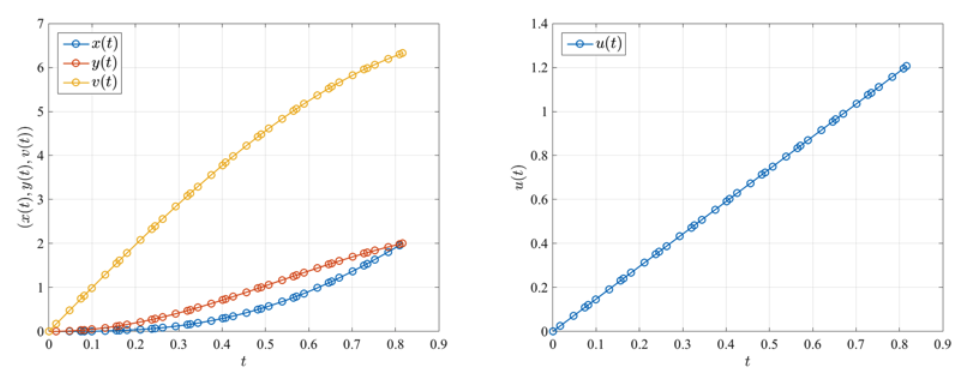
\includegraphics[width=0.9\linewidth]{figures/4_LODESTAR/Brachistochrone}
	\caption{The solution to the Brachistochrone problem, solved in GPOPS-2\cite{Rao2010}.}
	\label{fig:Brachistochrone}
\end{figure}




\textcolor{red}{\section{Example - Space Shuttle Reentry}}
\textcolor{red}{XXX I havent been able to find any good trajectories for comparison, that offer me the ability to recreate them..}
\textcolor{red}{XXX this is not quite the same as the GPOPS example, more similar to my dynamics}

This section describes an optimised shuttle reentry trajectory problem, taken from the textbook 'Practical Methods for Optimal Control and Estimation Using Nonlinear Programming' by Betts\cite{Betts2009}, which has been simulated in GPOPS-2 to illustrate the capabilities of GPOPS-2 when applied to a complex aerodynamic problem of an existing vehicle. The optimisation of the space shuttle reentry is relevant due to the large flight regime and long time period being simulated, which leads to a complex, extremely sensitive optimal control problem\cite{Betts2009}, similar in a simplified manner to the problem being solved in this work. The shuttle reentry problem is highly nonlinear and intractable to simple optimisation methods\cite{Betts2009}, making it suitable for illustrating the robustness of GPOPS-2 for aerospace problems of this type. 
The space shuttle reentry problem aims to maximise crossrange during reentry, with two cases; unconstrained, and limited by a simple heating rate constraint. The example in this section uses the vehicle model exactly as defined by Betts\cite{Betts2009} for comparison purposes, however the problem is formulated in a simplified version of the coordinate system that is used in the rest of this work. 


\subsection{Problem Formulation}

The dynamics of the space shuttle are defined exactly similarly to those in the problem designed by Betts\cite{Betts2009}, using a simplified model that neglects the rotation of the Earth and the tangential component of gravity:

\begin{equation}
\dot{r} = v \sin \gamma,
\end{equation}

\begin{equation}
\dot{\xi} = \frac{v\cos \gamma \cos \zeta}{r \cos \phi},
\end{equation}

\begin{equation}
\dot{\phi} = \frac{v\cos\gamma\sin\zeta}{r},
\end{equation}
\begin{equation}
\dot{\gamma} = \frac{L \cos\eta}{mv} + (\frac{v}{r}-\frac{g}{v})\cos\gamma,
\end{equation}
\begin{equation}
\dot{v} = \frac{D}{m}-g\sin\gamma,
\end{equation}
\begin{equation}
\dot{\zeta} = \frac{L  \sin\eta}{mv \cos \gamma}-\frac{v}{r}\tan\phi\cos\gamma\cos\zeta.
\end{equation}

The aerodynamics of the vehicle are modelled using simple correlations, where $C_L = −0.20704 + 0.029244\alpha$, and $C_D = 0.07854 -0.61592\times10^{-2}\alpha^2 + 0.621408\times10^{-3}\alpha^3$. The density is modelled as exponentially decaying, $\rho = 1.2255708354e^{-h/7254}$, and the gravity is modelled by an inverse square law, $g = \frac{\mu}{r^2}$.
The space shuttle initial conditions are set as follows\cite{Betts2009}, to simulate the entry of the shuttle into the upper atmosphere:
\begin{table}[H]
	\centering
\begin{tabular}{c c}
  $h_0$ =  79248m, & $v_0$ = 7803m/s, \\ 
  $\gamma_0$ =  -1$^\circ$, & $\phi_0$ =  0$^\circ$,\\ 
 $\xi_0$ =  0$^\circ$, & $\zeta_0$ =  0$^\circ$,\\ 
\end{tabular} 
\end{table}
and the end conditions are set as follows\cite{Betts2009}, to match the terminal area energy management interface:
\begin{table}[H]
	\centering
	\begin{tabular}{ c c c}
		   $h_f$ =  24384m, &  $v_f$ =762m/s, & $\gamma_f$ =  -5$^\circ$.\\ 
		
		
	\end{tabular} 
\end{table}

The problem is set to maximise crossrange from the initial point, which in this case is equivalent to maximising latitude:

\begin{equation}
J = -\phi_f.
\end{equation}

\subsection{Unconstrained Result}
The shuttle rentry crossrange maximisation problem is optimised in GPOPS-2, with result time histories shown in Figures \ref{fig:SpaceShuttleNoq1} and \ref{fig:SpaceShuttleNoq2}. The shuttle follows a 'skipping' trajectory, with an initially large bank angle that changes the heading of the vehicle rapidly in the early stages of reentry. The skips serve to maximise the range of the space shuttle's flight, and they are controlled by the angle of attack of the vehicle. The solution computed in GPOPS-2 matches the result computed by Betts\cite{Betts2009}, with the shape of the trajectories being close to identical. A maximum crossrange of 34.18$^\circ$ is achieved, a difference of 0.11\% when compared to the solution computed by Betts\cite{Betts2009}. This result is indicative of the ability of GPOPS-2 to compute highly sensitive optimal control problems for aerospace vehicles. 


\begin{figure}[H]
\centering
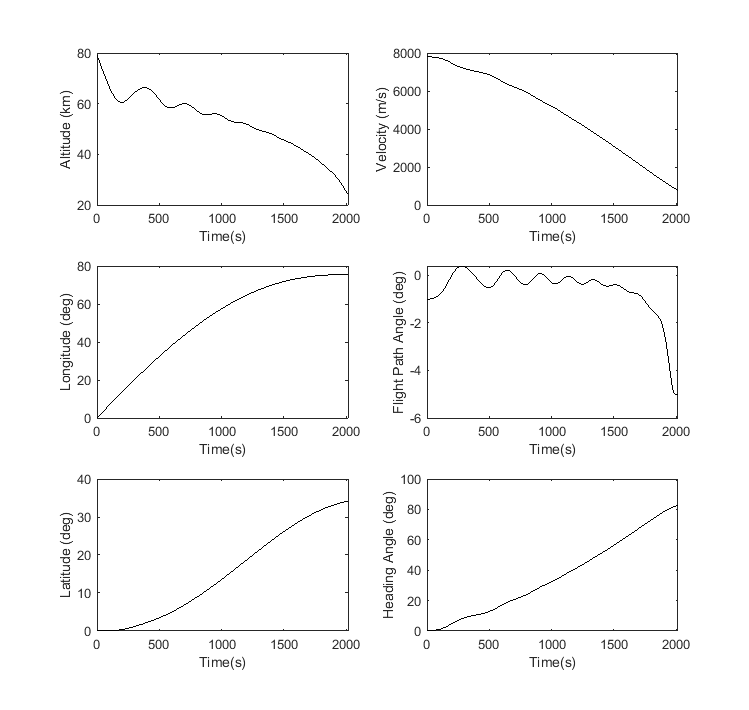
\includegraphics[width=0.7\linewidth]{figures/A1_uncertainty-analysis/SpaceShuttleNoq1}
\caption{}
\label{fig:SpaceShuttleNoq1}
\end{figure}
\begin{figure}[H]
\centering
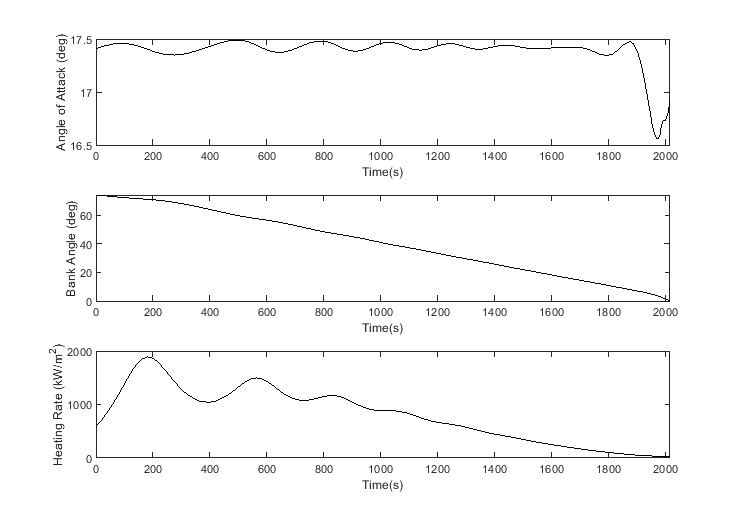
\includegraphics[width=0.7\linewidth]{figures/A1_uncertainty-analysis/SpaceShuttleNoq2}
\caption{}
\label{fig:SpaceShuttleNoq2}
\end{figure}


\subsection{Heating Rate Limited Result}
%\textcolor{red}{XXX Need to find a way to denote heating rate thats not q}
The heating rate of the space shuttle is limited during descent, to illustrate the ability of GPOPS-2 to deal with complex inequality constraints. The leading edge heating is approximated using a simplified empirical model, so that $q = q_aq_r$, where $q_r = 17700\sqrt{\rho}(0.0001v)^{3.07}$ and $q_a = 1.0672181 -0.19213774\times10^{-1}
\alpha + 0.21286289\times10^{-3}\alpha^2 -0.10117249\times10^{-5}\alpha^3$. The trajectory is successfully optimised in the presence of this complex inequality, once again showing a near identical trajectory to the optimised solution calculated by Betts\cite{Betts2009}. The maximum crossrange is reduced to 30.70$^\circ$, a difference of 0.25\% to the solution calculated by Betts\cite{Betts2009}.

\begin{figure}[H]
\centering
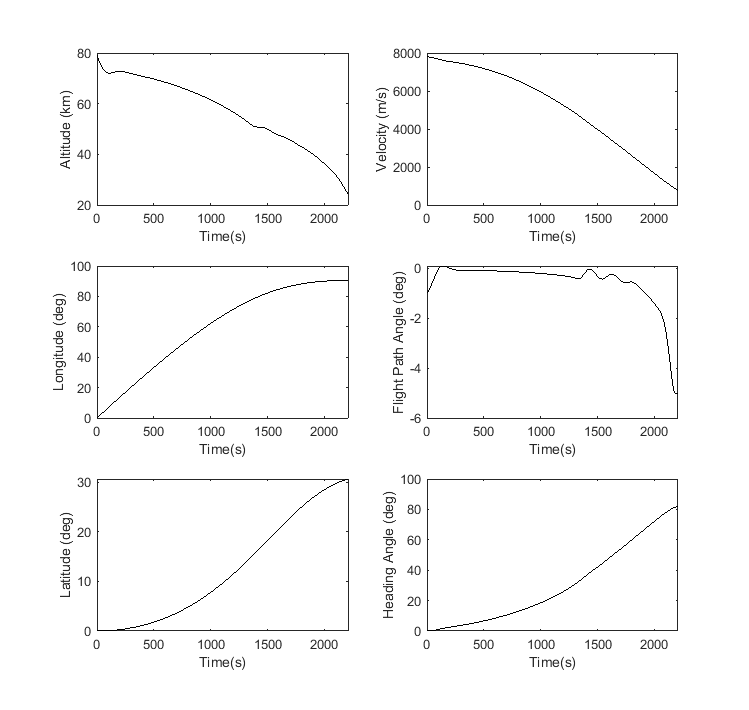
\includegraphics[width=0.7\linewidth]{figures/A1_uncertainty-analysis/SpaceShuttleq1}
\caption{}
\label{fig:SpaceShuttleq1}
\end{figure}
\begin{figure}[H]
\centering
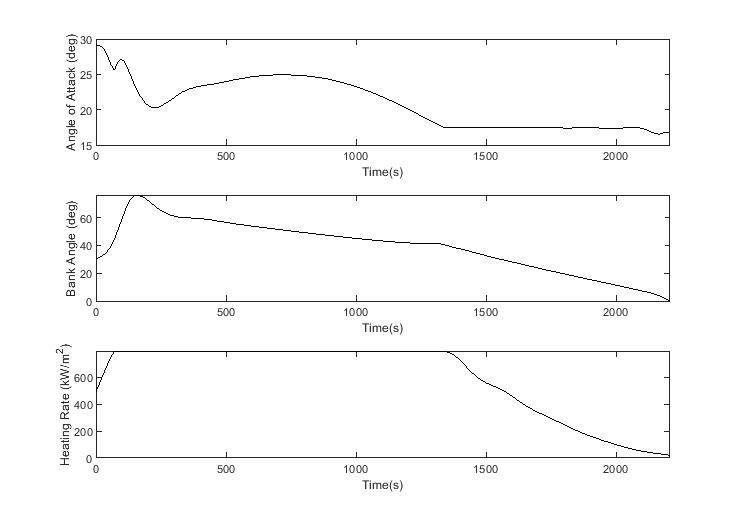
\includegraphics[width=0.7\linewidth]{figures/A1_uncertainty-analysis/SpaceShuttleq2}
\caption{}
\label{fig:SpaceShuttleq2}
\end{figure}


\section{Optimised Trajectory Verification}

\textcolor{red}{XXX Add verification here (possiblywith one of maddocks works, or a single stage to orbit, or space shuttle)}
\textcolor{red}{XXX  this is the section that descibes the error in 'timestep' as requested by reviewer, though there are multiple other factors. 'A Comparison of Accuracy and Computational E ciency of Three Pseudospectral Methods' also uses matlabs ODE45 for error comparison}.

\section{Optimised Trajectory Analysis}

This section presents an example of the convergence and verification of a trajectory optimised using GPOPS-2, within LODESTAR. The convergence and verification of a maximum payload-to-orbit trajectory solution, with SPARTAN fly-back (Case 11) is shown. 

\subsection{Mesh History}

\begin{figure}[ht]
	\centering
	\includegraphics[width=0.8\linewidth]{../LODESTAR_FINAL/Results/mode11/MeshHistory}
	\caption{The mesh history of each phase of the optimised, maximum payload-to-orbit trajectory with SPARTAN fly-back (Case 11). the phases are shown in each subfigure as follows: a) first stage rocket, b) SPARTAN acceleration, c) SPARTAN fly-back and d) third stage.}
	\label{fig:MeshHistory}
\end{figure}
The mesh history of the optimal trajectory solution is shown in Figure \ref{fig:MeshHistory}. The mesh is updated by GPOPS-2 in each iteration of the optimal solution. It can be observed that the meshes of the first and third stage rockets contain significantly less node points at the final iteration than the meshes of the SPARTAN's acceleration and return. This is due to the relatively simple dynamics and shorter flight time of the first and third stages. The first stage shows a cluster of nodes at the beginning of its trajectory, in the subsonic, transonic and low Mach regimes. In this region, the aerodynamics are changing rapidly, and the nodes are clustered to accurately capture the dynamic behaviour of the vehicle. After transition occurs to supersonic flight, the aerodynamics and engine performance of the vehicle change more slowly, and the nodes become more widely spaced. In contrast, the acceleration of the SPARTAN shows significant node density throughout. The operation of the SPARTAN is complex, as the dynamics of the vehicle and the performance of the scramjet engines vary significantly, even during relatively level flight. For this reason, the nodes of the return flight show even greater density. The trajectory conditions change significantly as the SPARTAN performs skipping manoeuvres, and transitions through the various return phases, necessitating high node density to capture the vehicle dynamics, particularly between powered and unpowered flight. The trajectories of the SPARTAN also last for a significantly longer time than the rocket trajectories, requiring more total nodes to accurately capture the vehicle dynamics. The third stage shows the least nodes at the final mesh iteration, as the dynamics of the third stage are relatively simple. Some node  clustering is observed in the first part of the trajectory, where the atmospheric density is still significant. 



\subsection{Verification}

After a trajectory has been calculated, it must be verified to ensure that the optimal control solver has converged correctly. Details on this verification are provided in Section \ref{sec:verification}. Figure \ref{fig:HamiltonianStandard} shows the Hamiltonian time history for the optimised trajectory solution of Case 11. For an optimal solution to be found, the Hamiltonian should be equal to 0 at all points over every phase. In a practical solution, a Hamiltonian close to 0 is acceptable, which is observable over all phases in the optimised solution. The Hamiltonian is close to 0 at all points of the trajectory, indicating that an optimal solution has been found. 
\begin{figure}[ht]
	\centering
	\includegraphics[width=0.9\linewidth]{../LODESTAR_FINAL/Results/mode11/HamiltonianStandard}
	\caption{The Hamiltonian time history of each phase of the maximum payload-to-orbit optimised trajectory, with SPARTAN fly-back (Case 11).}
	\label{fig:HamiltonianStandard}
\end{figure}

The next step in the verification process is to ensure that the dynamic constraints of the optimal control problem holds across the entire solution, ie. $\dot{\textbf{x}}(t) = f[t,\textbf{x}(t),\textbf{u}(t)]$. This is the most important step in the verification process, which checks that the optimal control solver has converged correctly, so that the physical dynamics of the vehicle are being correctly represented by the polynomial approximations within GPOPS-2. The dynamic constraints are tested by first calculating the dynamics of each vehicle at every node of the solution, using the vehicle simulations. These dynamics are then integrated over time using trapezoidal integration, starting at the initial conditions of each phase. The integrated dynamics are then compared to the states of the optimised solution. If the dynamic constraints have been satisfied, then the integrated dynamics of the system will be equal to the state variables of the solution. The error in the dynamic constraints of each state are shown in Figure \ref{fig:VerificationStandard}, calculated as the difference between the integrated dynamics and each state variable, normalised to the range of the state variable. 
It can be observed that all errors in the dynamic constraints are very small. The error that is present is likely to be due to the inaccuracies of the trapezoidal method, which is significantly less accurate than the approximating polynomials of the pseudospectral method. 



\begin{figure}[ht]
	\centering
	\includegraphics[width=0.9\linewidth]{../LODESTAR_FINAL/Results/mode11/VerificationStandard}
	\caption{The error between the integrated dynamics of the system, and the solution states of each phase of the maximum payload-to-orbit optimised trajectory, with SPARTAN fly-back (Case 11). Normalised to the range of each state.}
	\label{fig:VerificationStandard}
\end{figure}

The final verification step is a forward simulation of each phase. This forward simulation compares the solution state with a simulation which is forward integrated using only the controls of each stage. This is the most stringent method of checking the validity of the solution dynamics. However, it is expected that this verification will have significantly higher errors than the check which verifies the dynamics of each state independently, as the interdependencies of each state come into play, and small errors are compounded. Figure \ref{fig:ForwardErrorStandard} shows the error between the forward simulation and the solution states. As described in Section \ref{sec:verification}, the forward simulation of the return flight is separated into three segments, at 1/6th and 1/3rd of the flight time. The errors in the forward simulation of each stage are observed to be acceptably small, significantly under 1\% in all cases, and it is evident that compounding errors are the cause of the most extreme deviations. 

\begin{figure}[ht]
	\centering
	\includegraphics[width=0.9\linewidth]{../LODESTAR_FINAL/Results/mode11/ForwardErrorStandard}
	\caption{The error between the forward simulated states, and the solution states of each phase of the maximum payload-to-orbit optimised trajectory, with SPARTAN fly-back (Case 11). Normalised to the range of each state.}
	\label{fig:ForwardErrorStandard}
\end{figure}



\chapter{Modelling and Simulation}\label{Appendix:sim}
\section{Propulsion Interpolation Scheme}

\begin{figure}[ht]
	\centering
	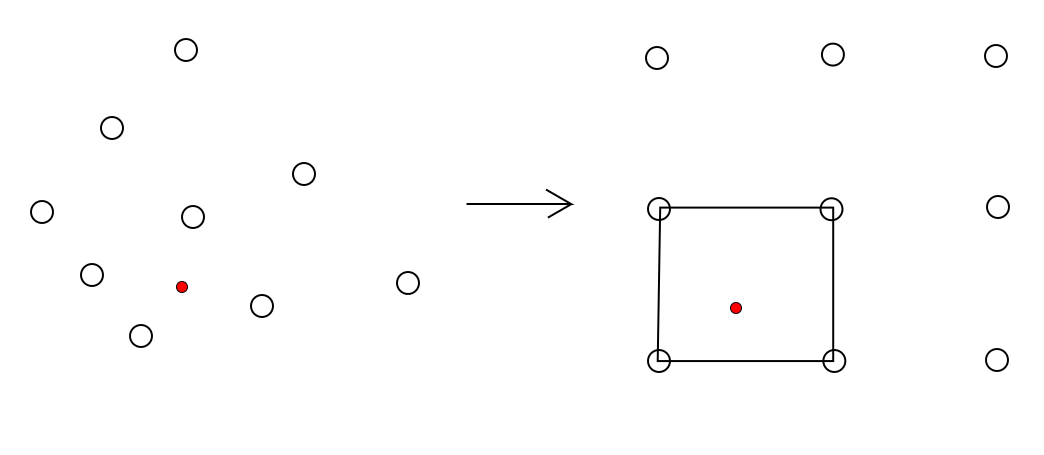
\includegraphics[width=0.8\linewidth]{figures/A1_uncertainty-analysis/interp}
	\caption{The transformation to a normalised interpolation scheme.}
	\label{fig:interp}
\end{figure}
This section describes the interpolation scheme used for the C-RESTM10 database to determine specific impulse.
The C-RESTM10 engine database consists of a set of engine conditions, including specific impulse, ordered by the inlet Mach number and temperature. This data set must be interpolated, to calculate the performance of the engine at each flight condition. However, no inlet Mach number and temperature values are repeated between any of the C-RESTM10 data points. This makes for a scattered data set which complicates the process of interpolating for specific impulse. It was observed that when interpolating for specific impulse, a scattered interpolation produces particularly poor results, and that fitting splines to the data set is the only way to produce an appropriate interpolation scheme. However, even when splines were fit, and the general trends of the specific impulse were matched, minuscule oscillations were still present in the interpolated values. These oscillations do not significantly affect a forward simulation, however, when using the vehicle model as part of an optimal control calculation, they can affect the convergence process. Consequently, it was necessary to craft a bespoke interpolation scheme in order to accurately interpolate the specific impulse of the vehicle. 

This interpolation begins by designating a new coordinate system, normalised to [0 1], running from data point with the lowest inlet temperature [0,0], to the data point with the highest inlet temperature [1,1]. Each data point is then given a set of normalised coordinates, and a cubic spline is fit to this set of normalised points using MATLAB's \textsf{griddedInterpolant} function. The normalised, orderd, data set ensures that this cubic spline is smooth, with no oscillations present. In order to interpolate at a specific location, each data point bounding the interpolation region is set as the corner of a square of data points in normalised coordinates. This is illustrated in Figure \ref{fig:interp}. The distance to each of these bounding data points is calculated, and the location to be interpolated is assigned a set of normalised coordinates. This set of normalised coordinates is used to interpolate for specific impulse. 

This process is accurate, but computationally time consuming, and would increase the computation time of the optimisation process significantly if implemented directly within the vehicle model.
 In order to expedite the interpolation process, interpolations are performed for the specific impulse for every combination of inlet Mach number and temperature present in the C-RESM10 database. This creates a grid of interpolated data points, which includes all of the data points present in the C-RESTM10 database. This grid of interpolated specific impulse values is then used as a new data set, which is now in \textsf{meshgrid} form, by which the specific impulse is interpolated. A bivariate spline is fitted to this grid of data points, using MATLAB's \textsf{griddedInterpolant} function, which is accessed by the vehicle model to determine specific impulse during flight.  







\section{SPARTAN Flow Results}
\begin{figure}[ht]
	\centering
	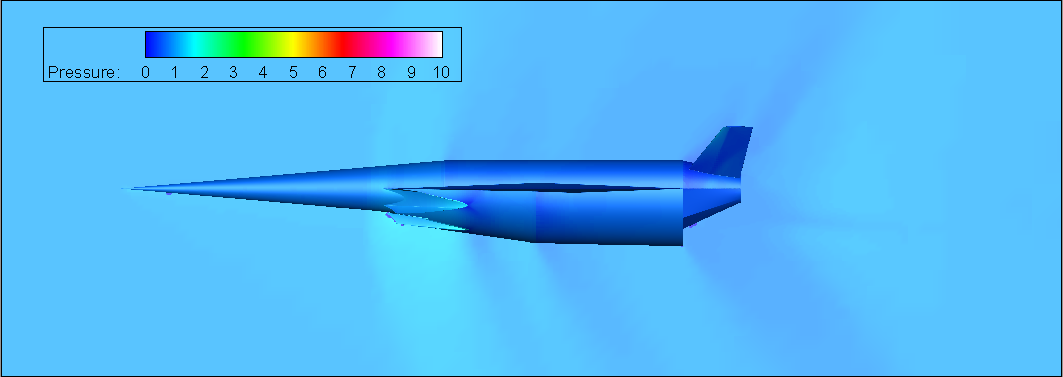
\includegraphics[width=0.9\linewidth]{figures/3_vehicle_design/M1p1AoA6}
	\caption{CART3D flow result for the SPARTAN, at Mach 1.1, 6$^\circ$ angle of attack.}
	\label{fig:M1}
\end{figure}
\begin{figure}[ht]
	\centering
	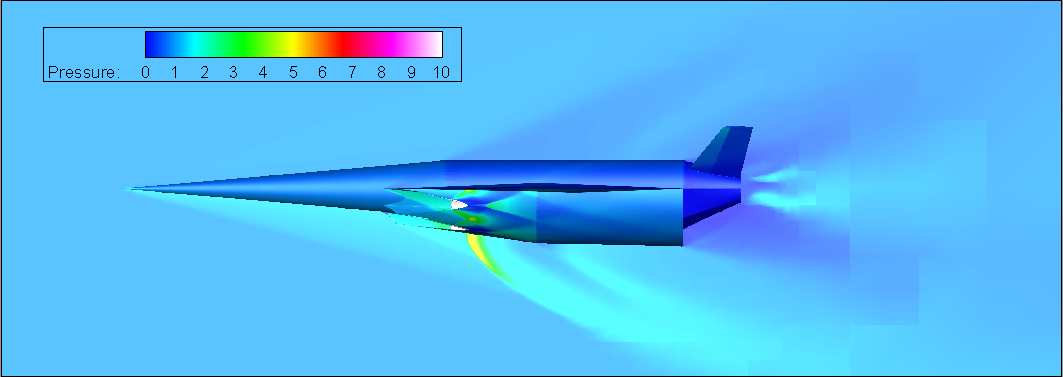
\includegraphics[width=0.9\linewidth]{figures/3_vehicle_design/M3AoA6}
	\caption{CART3D flow result for the SPARTAN, at Mach 3, 6$^\circ$ angle of attack.}
	\label{fig:M3AoA6}
\end{figure}
This section shows additional flow results for the SPARTAN, calculated using Cart3D.
Figures \ref{fig:M1} and \ref{fig:M3AoA6} show flow results for the SPARTAN, at Mach numbers of 1.1 and 3 respectively. It can be observed that at Mach 1.1, the bow shock is not significant, and the shock structure that is evident at higher speeds has not yet formed. At Mach 3, the unstarted C-REST engines are evident, causing significant amounts of the air entering the inlet to be expelled. Shock-shock interaction structures are evident on the cowl of the engines, causing areas of localised high pressure.


\FloatBarrier
\section{Cart3D Mesh}
\begin{figure}[ht]
	\centering
	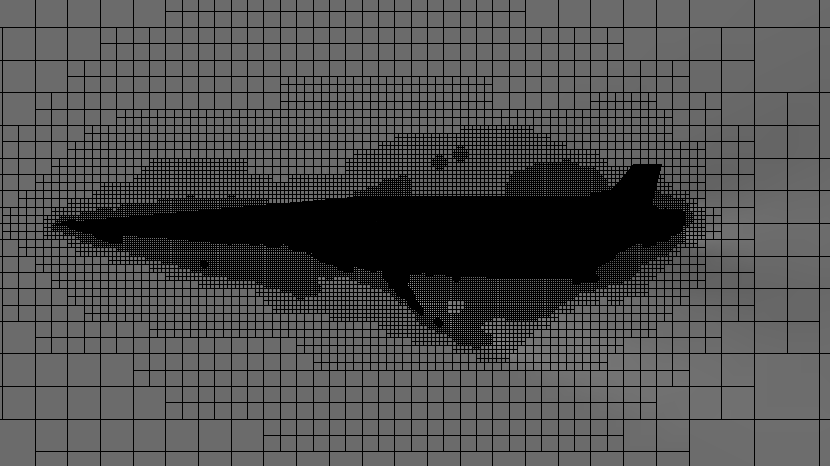
\includegraphics[width=0.7\linewidth]{figures/3_vehicle_design/M3AoA6GRID}
	\caption{Adapted mesh of the SPARTAN at Mach 6 3$^\circ$ angle of attack.}
	\label{fig:M3AoA6GRID}
\end{figure}

\begin{figure}[ht]
	\centering
	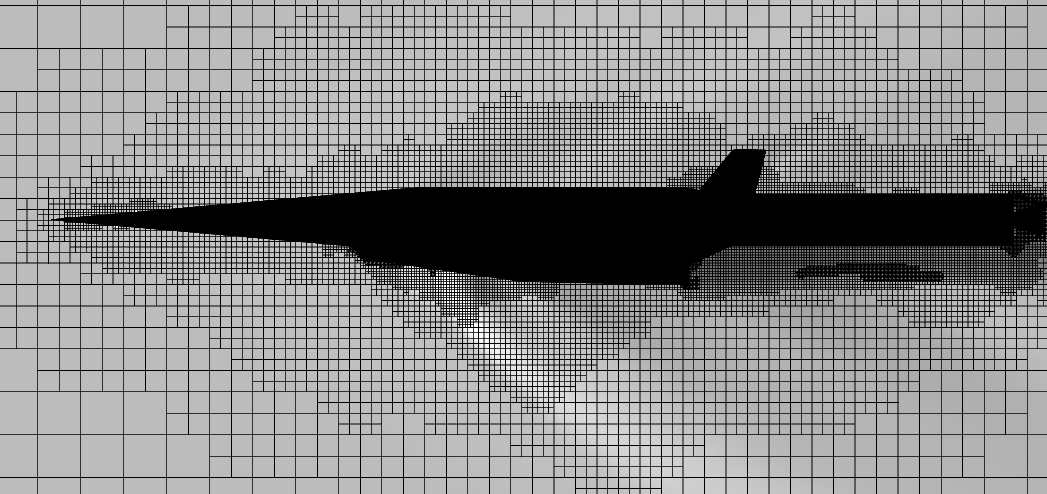
\includegraphics[width=0.7\linewidth]{figures/3_vehicle_design/CARTmesh}
	\caption{Adapted mesh around the SPARTAN and first stage vehicles, flying at Mach 2, -1$^\circ$ angle of attack.}
	\label{fig:CARTmesh}
\end{figure}
This section illustrates the converged meshes used by Cart3D.
Figures \ref{fig:M3AoA6GRID} and \ref{fig:CARTmesh} show adapted meshes for Cart3D solutions of the SPARTAN, and the SPARTAN and first stage. These meshes have been generated adaptively by Cart3D during the solution process. It can be observed that the mesh clusters around the vehicle, particularly in regions where strong shocks are present, where the mesh clusters at the shock front. 



\FloatBarrier
\section{Performance of the SPARTAN During Fly-Back}
Figure \ref{fig:returnIspStandard} shows the performance of the SPARTAN during the boost phase, described in Section \ref{sec:boost}. 

\begin{figure}[ht]
	\centering
	\includegraphics[width=0.7\linewidth]{../LODESTAR_FINAL/Results/mode11/returnIspStandard}
	\caption{The performance of the SPARTAN during the boost phase. Light blue indicates that the scramjet engines are turned on.}
	\label{fig:returnIspStandard}
\end{figure}


		\chapter{Alternate Trajectory Cases}
		
		\section{Sensitivity Study for a Launcher Design Varied for Uncertainty}
		\textcolor{red}{XXX do a 'worst case' launcher design under uncertainty (not necessarily just bad payload, more varied a lot) and show that sensitivity study still holds.}
		
		\section{Trajectory With Variation in Return Drag}
		I should maybe do a variation of just the return drag - "the performance of the launch system may be significantly different on the ascent and return trajectories (in addition to the engine flowpaths)"
		
		\section{Maximum Payload-To-Orbit Trajectory With Dynamic Pressure Constraint}\label{sec:Appendix_qconst}
		\textcolor{red}{XXX update this, make sure to update values too, used in ascent section}
		The maximum payload-to-orbit trajectory of the launch system with no SPARTAN fly-back (Case 2) was found to involve a significant altitude raising manoeuvre in the middle of the acceleration trajectory of the SPARTAN. Discerning the benefits of this altitude raising manoeuvre proved complex, requiring a trajectory to be calculated in which the altitude raising manoeuvre is prevented from occurring. This section describes an optimised trajectory in which the middle section of the SPARTAN's acceleration is constrained to flight at maximum dynamic pressure. 
		
		 This trajectory was optimised for maximum payload-to-orbit, with a 50kPa dynamic constraint between Mach numbers of 6 and 8, the region in which the altitude raising manoeuvre was observed to occur. This constraint successfully removed the altitude raising manoeuvre from the maximum payload-to-orbit optimised trajectory, allowing for a comparison to be made to quantify the benefits of the altitude raising manoeuvre. This comparison is made in Section \ref{sec:optimisednoreturn}. Figures \ref{fig:FirstStageqConstrained68},  \ref{fig:SecondStageqConstrained68} and \ref{fig:ThirdStageqConstrained68} show the maximum payload-to-orbit trajectory constrained to 50kPa between Mach numbers 6 to 8, and Table \ref{tab:constrained68} details key parameters of the trajectory. 
		
	\begin{table}[ht]
	\centering
\begin{tabular}{l c } 
	\hline \textbf{Trajectory Condition}
	& Value

	\\
	\hline \textbf{Payload to Orbit (kg)}
	& \textbf{\PayloadToOrbitqconstrainedNoReturn}
	\\
	\textbf{Total $\eta_{exergy}$ (\%)}
	& \textbf{\totalExergyEffqconstrainedNoReturn}
	\\
	\hline 
	\textbf{1$^{st}$ Stage $\eta_{exergy}$ (\%)}
	& \textbf{\firstExergyEffqconstrainedNoReturn}
	\\
	\textbf{Separation Alt, 1$\rightarrow$2 (km)}
	& \firstsecondSeparationAltqconstrainedNoReturn
	\\
	\textbf{Separation v, 1$\rightarrow$2 (m/s)}
	& \firstsecondSeparationvqconstrainedNoReturn
	\\
	\textbf{Separation $\gamma$, 1$\rightarrow$2 (deg)}
	& \firstsecondSeparationgammaqconstrainedNoReturn
	\\
	\hline 
	\textbf{2$^{nd}$ Stage $\eta_{exergy}$ (\%)}
	& \textbf{\secondExergyEffqconstrainedNoReturn}
	\\
	\textbf{Separation Alt, 2$\rightarrow$3 (km)}
	& \secondthirdSeparationAltqconstrainedNoReturn
	\\
	\textbf{Separation $v$, 2$\rightarrow$3 (m/s)}
	& \secondthirdSeparationvqconstrainedNoReturn
	\\
	\textbf{Separation $\gamma$, 2$\rightarrow$3 (deg)}
	& \secondthirdSeparationgammaqconstrainedNoReturn
	\\
	\textbf{2$^{nd}$ Stage Flight Time (s)}
	& \secondFlightTimeqconstrainedNoReturn
	\\
	\textbf{2$^{nd}$ Stage Distance Flown (km)}
	& \SecondDistqconstrainedNoReturn
	\\
	\hline 
	\textbf{3$^{rd}$ Stage $\eta_{exergy}$ (\%)}
	& \textbf{\thirddExergyEffqconstrainedNoReturn}
	\\
	\textbf{3$^{rd}$ Stage $t$, $q >$ 5kpa (s)}
	& \thirdqOverFiveqconstrainedNoReturn
	\\
	\textbf{3$^{rd}$ Stage Fuel Mass (kg)}
	& \thirdmFuelqconstrainedNoReturn
	\\
	\hline 
\end{tabular} 
\caption{A summary of key results from the maximum payload-to-orbit trajectory, constrained to 50kPa between Mach numbers 6 to 8.}
\label{tab:constrained68}

	\end{table}
		
\begin{figure}[th]
\centering
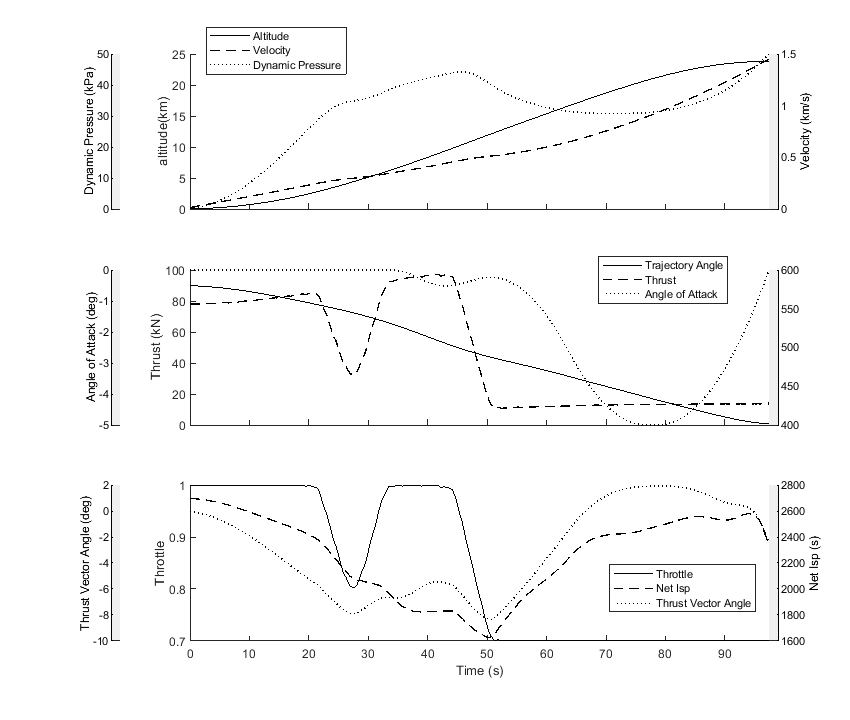
\includegraphics[width=0.9\linewidth]{../LODESTAR_FINAL/Results/10-qconstrained/FirstStageConstq}
\caption{The optimised maximum payload-to-orbit trajectory of the launch system constrained to 50kPa between Mach numbers 6 to 8, under power of the first stage rocket.}
\label{fig:FirstStageqConstrained68}
\end{figure}
		
\begin{figure}[th]
\centering
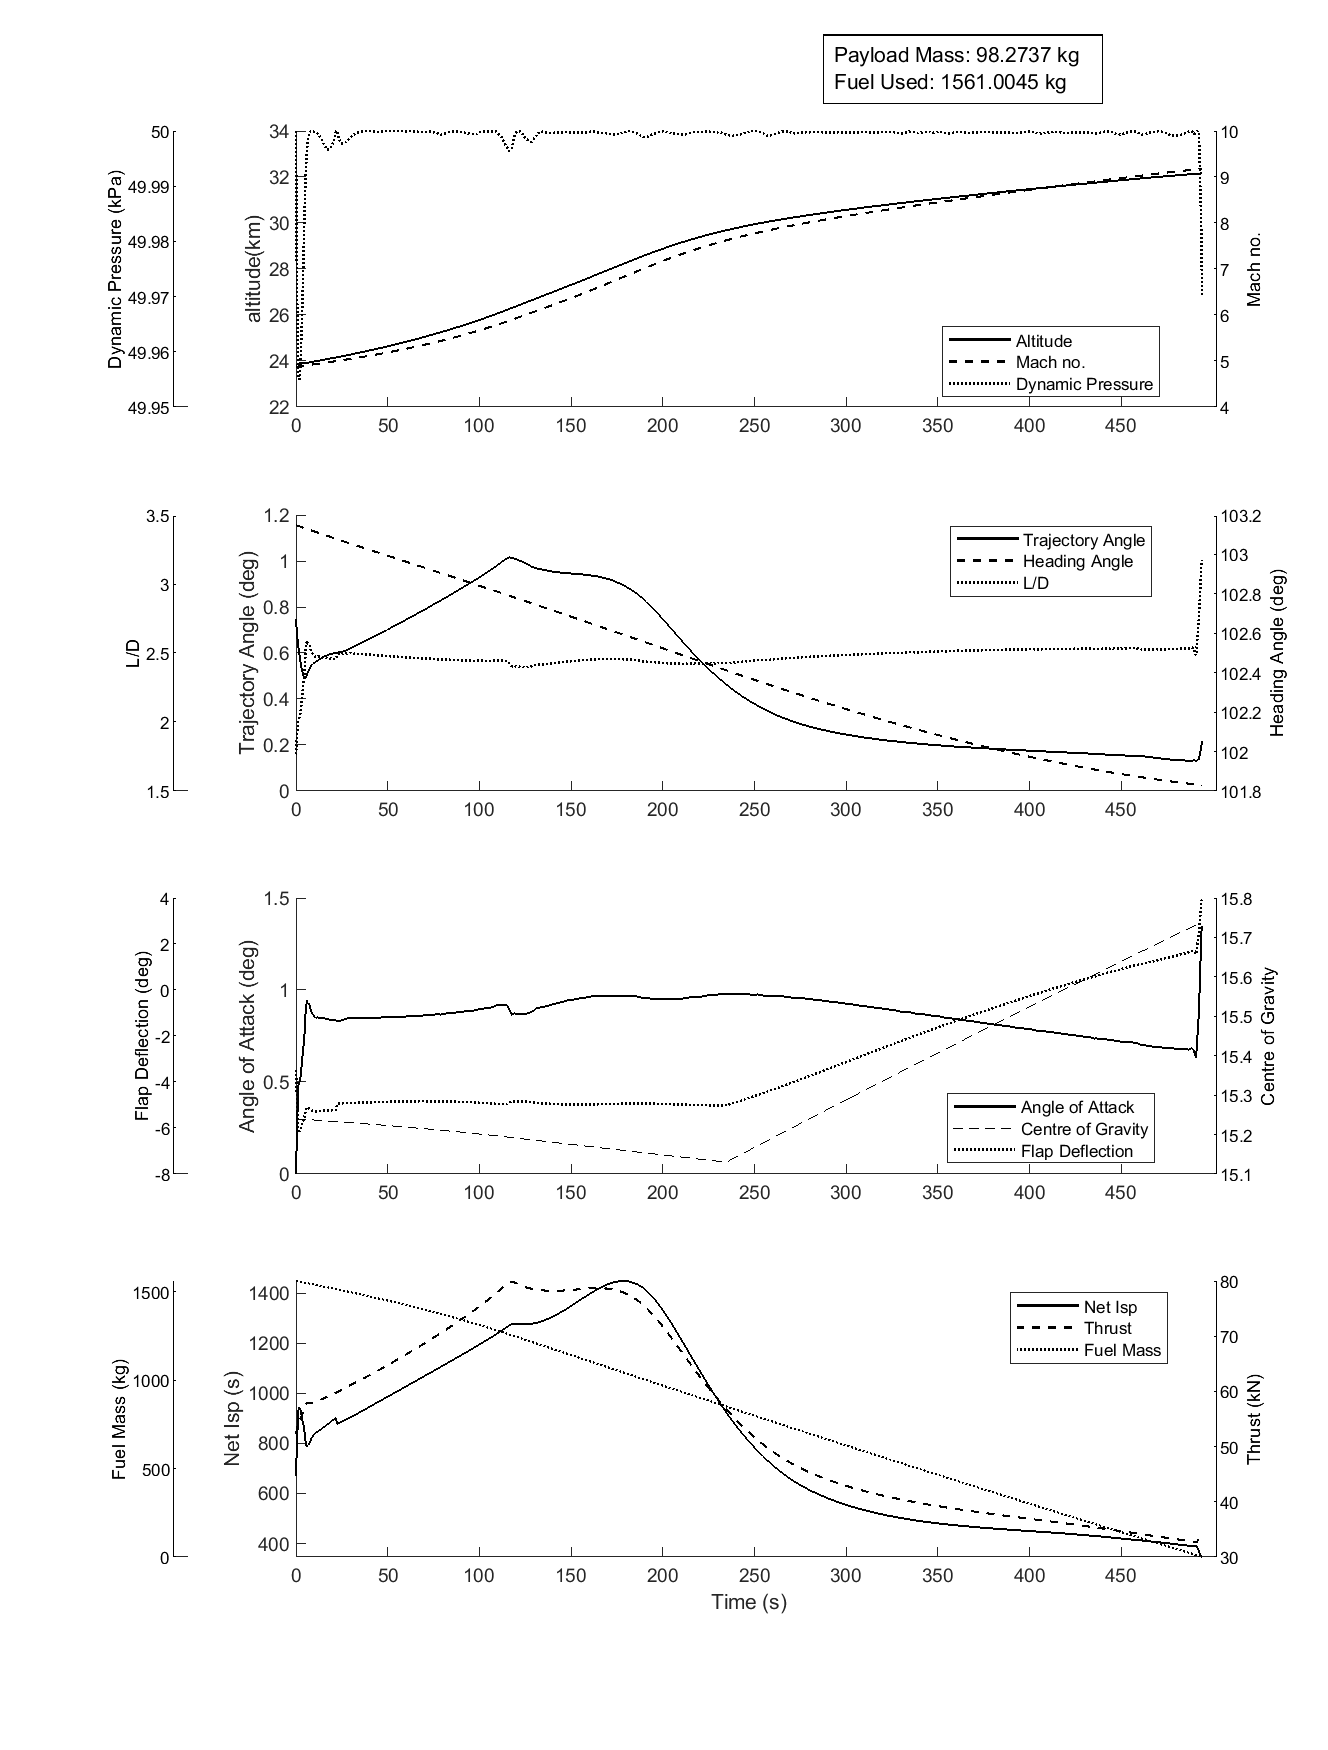
\includegraphics[width=0.9\linewidth]{../LODESTAR_FINAL/Results/10-qconstrained/SecondStageConstq}
\caption{The optimised maximum payload-to-orbit trajectory of the SPARTAN, constrained to 50kPa between Mach numbers 6 to 8.}
\label{fig:SecondStageqConstrained68}
\end{figure}

\begin{figure}[th]
\centering
\includegraphics[width=0.9\linewidth]{../LODESTAR_FINAL/Results/10-qconstrained/ThirdStageConstq}
\caption{The third stage trajectory of the launch system flying the maximum payload-to-orbit trajectory, constrained to 50kPa between Mach numbers 6 to 8.}
\label{fig:ThirdStageqConstrained68}
\end{figure}






\section{Constant Dynamic Pressure Trajectory with Fly-Back}
\textcolor{red}{XXX from 901 trajectory case, for heat shield reduction study}


\section{Sonic Boom Ground Effects}
\textcolor{red}{XXX update this}


\begin{figure}[ht]
	\centering
	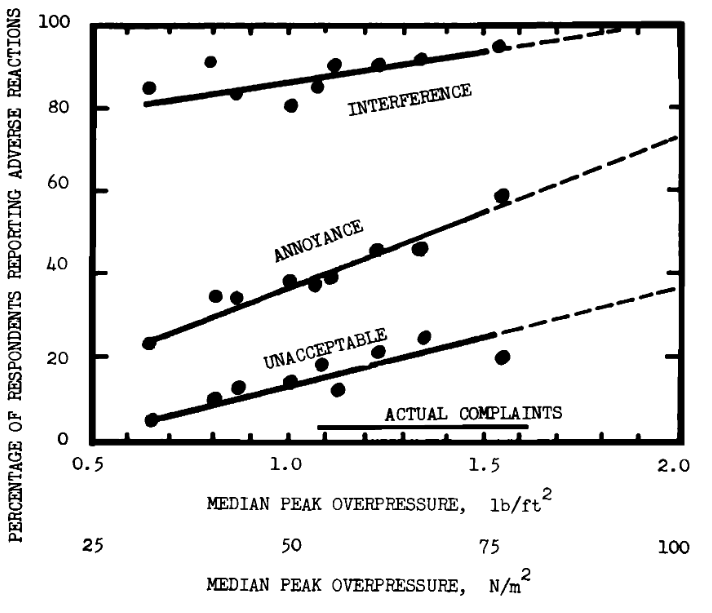
\includegraphics[width=0.6\linewidth]{figures/6_FlyBack/OverPressureResponse}
	\caption{The level of population annoyance with increasing overpressure.}
	\label{fig:OverPressureResponse}
\end{figure}

The flight of a hypersonic vehicle has the potential to create significant overpressures on the ground due to sonic booms. This section describes the effects of the sonic booms generated by the SPARTAN. 

Even when a hypersonic vehicle is flying at high altitudes, the overpressures on the ground may still be large enough to have detrimental effects on any populated areas being overflown. The overpressure from sonic booms can cause significant annoyance to the populace, or in more extreme cases, long term damage to building structures or peoples health. 
When the SPARTAN is launched to a sun synchronous orbit from the Equatorial Launch Australia launch site, it flies over a significant portion of Papua. Fortunately, Papua is sparsely populated, and the number of towns flown over by the SPARTAN will be low. However the effects on these population centres may still be significant. In order to assess the impact of the SPARTAN's flight, the magnitude of the overpressure from its sonic booms must be calculated. 
\begin{figure}[ht]
	\centering
	\includegraphics[width=0.9\linewidth]{../LODESTAR_FINAL/Results/mode11/OverPressureStandard}
	\caption{The sonic boom overpressure on the ground, for the optimised trajectory path (Case 11).}
	\label{fig:OverPressureStandard}
\end{figure}

The sonic boom overpressures are estimated using the 'first cut' estimation technique \cite{Carlson1972}. This estimation technique can approximate sonic boom overpressures moderately well, and is useful as a first approximation to the sonic boom overpressures generated by an aerospace vehicle. The overpressures generated by the SPARTAN are calculated over its trajectory, shown in Figure \ref{fig:OverPressureStandard}. It is found that overpressures of up to 375.3Pa occur during flight over land during the maximum payload-to-orbit trajectory of the SPARTAN. These overpressures have a low but significant probability of causing cosmetic damage to structures (~1.5\% for plaster and ~0.4\% for glass)\cite{Hershey1976}. In addition, overpressures of these magnitudes have been rated as unacceptably annoying to the majority populace being overflown, as shown in Figure \ref{fig:OverPressureResponse}. 
These overpressures indicate that overflight of populated areas may not be reasonable for the SPARTAN flying its maximum payload-to-orbit trajectory path, with fly-back (Case 11). 


%http://www.dtic.mil/dtic/tr/fulltext/u2/a028512.pdf





\section{Alternate Launch Location}
\textcolor{red}{XXX update this}

In this section, an alternate southerly launch is investigated for the rocket-scramjet-rocket launch system, in the case that flight over Papua is not possible. This launch occurs from Streaky Bay, the possible location of a launch site being developed by Southern Launch Australia\cite{Council2016}. The maximum payload-to-orbit has been calculated from this launch site using LODESTAR. Figure \ref{fig:GroundTrackAlternate} shows the ground track of this optimised trajectory, and Table \ref{tab:summaryalternate} details a summary of the key trajectory parameters. The shape of this optimised trajectory is very similar to the optimal trajectory of the launch system launched from the Northern Territory (Case 11). The first stage initially pitches towards the west, separating the SPARTAN in a westerly direction. the SPARTAN then performs a banking manoeuvre to the south, and a pull-up before third stage release. After separation, the SPARTAN exhibits initial turn, boost-skip and approach phases during fly-back, with the scramjet engine igniting three times at the troughs of the first three skips, in the same manner as when launching northerly. A higher payload to orbit is achieved when launching from a southerly location, attaining a total of \PayloadToOrbitAlternate kg of payload-to-orbit, an increase of +2.9\% compared to northerly launch. This payload increase is caused by the rotation of the Earth hindering, rather than assisting, when launching into a retrograde orbit, making launch from a more southerly point desirable. 


\begin{figure}[th]
	\centering
	\includegraphics[width=1\linewidth]{../LODESTAR_FINAL/Results/mode01/GroundTrackAlternate}
	\caption{The optimised maximum payload-to-orbit trajectory of the launch system launching onto a southerly orbit, from Streaky Bay.}
	\label{fig:GroundTrackAlternate}
\end{figure}

\begin{table}
	\centering
	\begin{tabular}{l c} 
		\hline \textbf{Trajectory Condition}
		& Value

		\\
		\hline \textbf{Payload to Orbit (kg)}
		& \textbf{\PayloadToOrbitAlternate}
		\\
		\textbf{Total $\eta_{exergy}$ (\%)}
		& \textbf{\totalExergyEffAlternate}
		\\
		\hline 
		\textbf{1$^{st}$ Stage $\eta_{exergy}$ (\%)}
		& \textbf{\firstExergyEffAlternate}
		\\
		\textbf{Separation Alt, 1$\rightarrow$2 (km)}
		& \firstsecondSeparationAltAlternate
		\\
		\textbf{Separation v, 1$\rightarrow$2 (m/s)}
		& \firstsecondSeparationvAlternate
		\\
		\textbf{Separation $\gamma$, 1$\rightarrow$2 (deg)}
		& \firstsecondSeparationgammaAlternate
		\\
		\hline 
		\textbf{2$^{nd}$ Stage $\eta_{exergy}$ (\%)}
		& \textbf{\secondExergyEffAlternate}
		\\
		\textbf{Separation Alt, 2$\rightarrow$3 (km)}
		& \secondthirdSeparationAltAlternate
		\\
		\textbf{Separation $v$, 2$\rightarrow$3 (m/s)}
		& \secondthirdSeparationvAlternate
		\\
		\textbf{Separation $\gamma$, 2$\rightarrow$3 (deg)}
		& \secondthirdSeparationgammaAlternate
		\\
		\textbf{2$^{nd}$ Stage Flight Time (s)}
		& \secondFlightTimeAlternate
		\\
		\textbf{2$^{nd}$ Stage Distance Flown (km)}
		& \SecondDistAlternate
		\\
		\textbf{2$^{nd}$ Stage Return Fuel (kg)}
		& \returnFuelAlternate
		\\
		\textbf{2$^{nd}$ Stage Return Distance (km)}
		& \returnDistAlternate
		\\
		\hline 
		\textbf{3$^{rd}$ Stage $\eta_{exergy}$ (\%)}
		& \textbf{\thirddExergyEffAlternate}
		\\
		\textbf{3$^{rd}$ Stage $t$, $q >$ 5kpa (s)}
		& \thirdqOverFiveAlternate
		\\
		\textbf{3$^{rd}$ Stage Fuel Mass (kg)}
		& \thirdmFuelAlternate
		\\
		\hline 
	\end{tabular} 
	\caption{A summary of key trajectory parameters of the maximum payload-to-orbit trajectory launched in a southerly direction.}
	\label{tab:summaryalternate}
\end{table}




		
		\chapter{Trajectory Plot Comparisons}\label{sec:Appendix_trajectorycomparisons}
		
		\textcolor{red}{XXX update these}
		
This section contains trajectory plot comparisons for the sensitivity studies performed in Section \ref{sec:sensitivityNoReturn} and \ref{sec:sensitivity}. Comparisons and analyses between these trajectories are performed in the relevant sections. 
		\clearpage
		\section{Optimised Ascent Trajectory Comparisons With No Fly-Back}
		
		\subsection{Case 3: Maximum Dynamic Pressure Sensitivity Comparison}\label{sec:app_comparison20}
		
		
\begin{figure}[!ht]
\centering
\includegraphics[width=1\linewidth]{../LODESTAR_FINAL/Results/mode20/SecondStageComparison}
\caption{Comparison of SPARTAN ascent trajectories with variation in the maximum dynamic pressure of the SPARTAN.}
\label{fig:SecondStageComparison1}
\end{figure}

\begin{figure}[!th]
\centering
\includegraphics[width=1\linewidth]{../LODESTAR_FINAL/Results/mode20/ThirdStageComparison}
\caption{Comparison of third stage rocket ascent trajectories with variation in the maximum dynamic pressure of the SPARTAN.}
\label{fig:ThirdStageComparison1}
\end{figure}
\FloatBarrier

\clearpage

\subsection{Case 4: SPARTAN Drag Sensitivity Comparison}\label{sec:app_comparison40}

\begin{figure}[!th]
\centering
\includegraphics[width=1\linewidth]{../LODESTAR_FINAL/Results/mode40/SecondStageComparison}
\caption{Comparison of SPARTAN ascent trajectories with variation in the drag of the SPARTAN.}
\label{fig:SecondStageComparison3}
\end{figure}

\begin{figure}[!th]
\centering
\includegraphics[width=1\linewidth]{../LODESTAR_FINAL/Results/mode40/ThirdStageComparison}
\caption{Comparison of third stage rocket ascent trajectories with variation in the drag of the SPARTAN.}
\label{fig:ThirdStageComparison3}
\end{figure}
\FloatBarrier
\clearpage
\subsection{Case 5: SPARTAN Specific Impulse Sensitivity Comparison}\label{sec:app_comparison30}


\begin{figure}[!th]
	\centering
	\includegraphics[width=1\linewidth]{../LODESTAR_FINAL/Results/mode30/SecondStageComparison}
	\caption{Comparison of SPARTAN ascent trajectories with variation in the specific impulse of the SPARTAN.}
	\label{fig:SecondStageComparison2}
	
\end{figure}
\begin{figure}[!th]
	\centering
	\includegraphics[width=1\linewidth]{../LODESTAR_FINAL/Results/mode30/ThirdStageComparison}
	\caption{Comparison of third stage rocket ascent trajectories with variation in the specific impulse of the SPARTAN.}
	\label{fig:ThirdStageComparison2}
\end{figure}
\FloatBarrier
\clearpage
\subsection{Case 6: SPARTAN Mass Sensitivity Comparison}\label{sec:app_comparison100}

\begin{figure}[!th]
\centering
\includegraphics[width=1\linewidth]{../LODESTAR_FINAL/Results/mode100/SecondStageComparison}
\caption{Comparison of SPARTAN ascent trajectories with variation in the mass of the SPARTAN.}
\label{fig:SecondStageComparison4}
\end{figure}

\begin{figure}[!th]
\centering
\includegraphics[width=1\linewidth]{../LODESTAR_FINAL/Results/mode100/ThirdStageComparison}
\caption{Comparison of third stage rocket ascent trajectories with variation in the mass of the SPARTAN.}
\label{fig:ThirdStageComparison4}
\end{figure}
\FloatBarrier
\clearpage
\subsection{Case 7: SPARTAN Fuel Mass Sensitivity Comparison}\label{sec:app_comparison110}
\begin{figure}[!th]
\centering
\includegraphics[width=1\linewidth]{../LODESTAR_FINAL/Results/mode110/SecondStageComparison}
\caption{Comparison of SPARTAN ascent trajectories with variation in the fuel mass of the SPARTAN.}
\label{fig:SecondStageComparison5}
\end{figure}

\begin{figure}[!th]
\centering
\includegraphics[width=1\linewidth]{../LODESTAR_FINAL/Results/mode110/ThirdStageComparison}
\caption{Comparison of third stage rocket ascent trajectories with variation in the fuel mass of the SPARTAN.}
\label{fig:ThirdStageComparison5}
\end{figure}
\FloatBarrier
\clearpage
\subsection{Case 8: Third Stage Mass Sensitivity Comparison}\label{sec:app_comparison80}

\begin{figure}[!th]
\centering
\includegraphics[width=1\linewidth]{../LODESTAR_FINAL/Results/mode80/SecondStageComparison}
\caption{Comparison of SPARTAN ascent trajectories with variation in the mass of the third stage.}
\label{fig:SecondStageComparison6}
\end{figure}


\begin{figure}[!th]
\centering
\includegraphics[width=1\linewidth]{../LODESTAR_FINAL/Results/mode80/ThirdStageComparison}
\caption{Comparison of third stage rocket ascent trajectories with variation in the mass of the third stage.}
\label{fig:ThirdStageComparison6}
\end{figure}

\FloatBarrier
\clearpage
\subsection{Case 9: Third Stage Specific Impulse Sensitivity Comparison}\label{sec:app_comparison90}

\begin{figure}[!th]
	\centering
	\includegraphics[width=1\linewidth]{../LODESTAR_FINAL/Results/mode90/SecondStageComparison}
	\caption{Comparison of SPARTAN ascent trajectories with variation in the specific impulse of the third stage.}
	\label{fig:SecondStageComparison7}
\end{figure}

\begin{figure}[!th]
\centering
\includegraphics[width=1\linewidth]{../LODESTAR_FINAL/Results/mode90/ThirdStageComparison}
\caption{Comparison of third stage rocket ascent trajectories with variation in the specific impulse of the third stage.}
\label{fig:ThirdStageComparison7}
\end{figure}
\FloatBarrier
\clearpage
\subsection{Case 10:Third Stage Drag Sensitivity Comparison}\label{sec:app_comparison70}

\begin{figure}[!th]
\centering
\includegraphics[width=1\linewidth]{../LODESTAR_FINAL/Results/mode70/SecondStageComparison}
\caption{Comparison of SPARTAN ascent trajectories with variation in the drag of the third stage.}
\label{fig:SecondStageComparison8}
\end{figure}


\begin{figure}[!th]
\centering
\includegraphics[width=1\linewidth]{../LODESTAR_FINAL/Results/mode70/ThirdStageComparison}
\caption{Comparison of third stage rocket ascent trajectories with variation in the drag of the third stage.}
\label{fig:ThirdStageComparison8}
\end{figure}

\FloatBarrier
\clearpage
\section{Optimised Ascent Trajectory Comparisons With Fly-Back}
\FloatBarrier
\subsection{Case 12: Dynamic Pressure Sensitivity Comparison}\label{sec:app_comparison21}
\begin{figure}[!th]
\centering
\includegraphics[width=1\linewidth]{../LODESTAR_FINAL/Results/mode21/SecondStageComparison}
\caption{Comparison of SPARTAN ascent trajectories with variation in the maximum dynamic pressure of the SPARTAN.}
\label{fig:SecondStageComparison9}
\end{figure}

\begin{figure}[!th]
\centering
\includegraphics[width=1\linewidth]{../LODESTAR_FINAL/Results/mode21/ThirdStageComparison}
\caption{Comparison of third stage rocket ascent trajectories with variation in the maximum dynamic pressure of the SPARTAN.}
\label{fig:ThirdStageComparison9}
\end{figure}

\begin{figure}[!th]
\centering
\includegraphics[width=1\linewidth]{../LODESTAR_FINAL/Results/mode21/ReturnComparison}
\caption{Comparison of SPARTAN return trajectories with variation in the maximum dynamic pressure of the SPARTAN.}
\label{fig:ReturnComparison}
\end{figure}



\FloatBarrier
\clearpage
\subsection{Case 13: SPARTAN Drag Sensitivity Comparison}\label{sec:app_comparison41}
\begin{figure}[!th]
\centering
\includegraphics[width=1\linewidth]{../LODESTAR_FINAL/Results/mode41/SecondStageComparison}
\caption{Comparison of SPARTAN ascent trajectories with variation in the drag of the SPARTAN.}
\label{fig:SecondStageComparison11}
\end{figure}

\begin{figure}[!th]
\centering
\includegraphics[width=1\linewidth]{../LODESTAR_FINAL/Results/mode41/ThirdStageComparison}
\caption{Comparison of third stage rocket ascent trajectories with variation in the drag of the SPARTAN.}
\label{fig:ThirdStageComparison11}
\end{figure}

\begin{figure}[!th]
\centering
\includegraphics[width=1\linewidth]{../LODESTAR_FINAL/Results/mode41/ReturnComparison}
\caption{Comparison of SPARTAN return trajectories with variation in the drag of the SPARTAN.}
\label{fig:ReturnComparison11}
\end{figure}

\FloatBarrier
\clearpage
\subsection{Case 14:SPARTAN Specific Impulse Sensitivity Comparison}\label{sec:app_comparison31}
\begin{figure}[!th]
	\centering
	\includegraphics[width=1\linewidth]{../LODESTAR_FINAL/Results/mode31/SecondStageComparison}
	\caption{Comparison of SPARTAN ascent trajectories with variation in the specific impulse of the SPARTAN.}
	\label{fig:SecondStageComparison10}
\end{figure}

\begin{figure}[!th]
	\centering
	\includegraphics[width=1\linewidth]{../LODESTAR_FINAL/Results/mode31/ThirdStageComparison}
	\caption{Comparison of third stage rocket ascent trajectories with variation in the specific impulse of the SPARTAN.}
	\label{fig:ThirdStageComparison10}
\end{figure}

\begin{figure}[!th]
	\centering
	\includegraphics[width=1\linewidth]{../LODESTAR_FINAL/Results/mode31/ReturnComparison}
	\caption{Comparison of SPARTAN return trajectories with variation in the specific impulse of the SPARTAN.}
	\label{fig:ReturnComparison10}
\end{figure}
\FloatBarrier
\clearpage
\subsection{Case 15: SPARTAN Mass Sensitivity Comparison}\label{sec:app_comparison101}

\begin{figure}[!th]
\centering
\includegraphics[width=1\linewidth]{../LODESTAR_FINAL/Results/mode101/SecondStageComparison}
\caption{Comparison of SPARTAN ascent trajectories with variation in the mass of the SPARTAN.}
\label{fig:SecondStageComparison12}
\end{figure}

\begin{figure}[!th]
\centering
\includegraphics[width=1\linewidth]{../LODESTAR_FINAL/Results/mode101/ThirdStageComparison}
\caption{Comparison of third stage rocket ascent trajectories with variation in the mass of the SPARTAN.}
\label{fig:ThirdStageComparison12}
\end{figure}

\begin{figure}[!th]
\centering
\includegraphics[width=1\linewidth]{../LODESTAR_FINAL/Results/mode101/ReturnComparison}
\caption{Comparison of SPARTAN return trajectories with variation in the mass of the SPARTAN.}
\label{fig:ReturnComparison12}
\end{figure}

\FloatBarrier
\clearpage
\subsection{Case 16: SPARTAN Fuel Mass Sensitivity Comparison}\label{sec:app_comparison111}

\begin{figure}[!th]
\centering
\includegraphics[width=1\linewidth]{../LODESTAR_FINAL/Results/mode111/SecondStageComparison}
\caption{Comparison of SPARTAN ascent trajectories with variation in the fuel mass of the SPARTAN.}
\label{fig:SecondStageComparison13}
\end{figure}

\begin{figure}[!th]
\centering
\includegraphics[width=1\linewidth]{../LODESTAR_FINAL/Results/mode111/ThirdStageComparison}
\caption{Comparison of third stage rocket ascent trajectories with variation in the fuel mass of the SPARTAN.}
\label{fig:ThirdStageComparison13}
\end{figure}

\begin{figure}[!th]
\centering
\includegraphics[width=1\linewidth]{../LODESTAR_FINAL/Results/mode111/ReturnComparison}
\caption{Comparison of SPARTAN return trajectories with variation in the fuel mass of the SPARTAN.}
\label{fig:ReturnComparison13}
\end{figure}


\FloatBarrier
\clearpage
\subsection{Case 17: Third Stage Mass Sensitivity Comparison}\label{sec:app_comparison81}
\begin{figure}[!th]
\centering
\includegraphics[width=1\linewidth]{../LODESTAR_FINAL/Results/mode81/SecondStageComparison}
\caption{Comparison of SPARTAN ascent trajectories with variation in the mass of the third stage.}
\label{fig:SecondStageComparison14}
\end{figure}

\begin{figure}[!th]
\centering
\includegraphics[width=1\linewidth]{../LODESTAR_FINAL/Results/mode81/ThirdStageComparison}
\caption{Comparison of third stage rocket ascent trajectories with variation in the mass of the third stage.}
\label{fig:ThirdStageComparison14}
\end{figure}



\begin{figure}[!th]
	\centering
	\includegraphics[width=1\linewidth]{../LODESTAR_FINAL/Results/mode81/ReturnComparison}
	\caption{Comparison of SPARTAN return trajectories with variation in the mass of the third stage.}
	\label{fig:ReturnComparison14}
\end{figure}
\FloatBarrier
\clearpage
\subsection{Case 18: Third Stage Specific Impulse Sensitivity Comparison}\label{sec:app_comparison91}

\begin{figure}[!th]
\centering
\includegraphics[width=1\linewidth]{../LODESTAR_FINAL/Results/mode91/SecondStageComparison}
\caption{Comparison of SPARTAN ascent trajectories with variation in the specific impulse of the third stage.}
\label{fig:SecondStageComparison15}
\end{figure}


\begin{figure}[!th]
\centering
\includegraphics[width=1\linewidth]{../LODESTAR_FINAL/Results/mode91/ThirdStageComparison}
\caption{Comparison of third stage rocket ascent trajectories with variation in the specific impulse of the third stage.}
\label{fig:ThirdStageComparison15}
\end{figure}


\begin{figure}[!th]
\centering
\includegraphics[width=1\linewidth]{../LODESTAR_FINAL/Results/mode91/ReturnComparison}
\caption{Comparison of SPARTAN return trajectories with variation in the specific impulse of the third stage.}
\label{fig:ReturnComparison15}
\end{figure}


\chapter{Viscous Drag Variation}
\textcolor{red}{XXX Will need to redo this with variation for all stages}

This section presents the sensitivity of the launch system performance to variations in the viscous drag of the SPARTAN. This sensitivity analysis is intended as a reference, to indicate the magnitude of variations in the viscous drag of the SPARTAN due to variations in modelling methods, and is unlikely to be indicative of any physical design variations.
The viscous drag component of the SPARTAN's aerodynamics is calculated using flat plate correlations, which require an estimation of the laminar to turbulent transition point on the body of the SPARTAN\cite{Ward2018}. This transition point is difficult to estimate to a high degree of accuracy, and can have a significant effect on the viscous drag of an aircraft\cite{Ward2018}.
The viscous drag component of the SPARTAN's aerodynamics is varied, in order to assess the impact of the viscous drag model used. Optimal trajectories are calculated with the viscous drag set at levels of 20\%, 50\%, 107\% and 115\% of the baseline, which correspond to the possible viscous drag range due to transition point variation. Table \ref{tab:viscous} details key trajectory parameters of the optimised trajectories, and Figures \ref{fig:SecondStageComparison-}, \ref{fig:ThirdStageComparison-} and \ref{fig:ReturnComparison-} show comparison plots of the optimised trajectories. The sensitivity of the launch system to the viscous drag of the SPARTAN is shown to be relatively low, as the deviations in the viscous drag model are expected to be small, relative to the range tested. This low sensitivity indicating that the modelling process of the viscous drag is unlikely to have a large effect on the accuracy of the maximum payload-to-orbit solution.

\begin{table}[ht]
	\centering
	\begin{tabular}{l c c c c c c} 
		\hline \textbf{Trajectory Condition} \qquad vC$_D$:
		&20\%
		&50\%
		&100\%
		&107\%
		&115\%
		& $\Delta/\Delta$\%vC$_D$
		\\
		\hline \textbf{Payload to Orbit (kg)}
		& \textbf{\PayloadToOrbitvCdTwenty}
		& \textbf{\PayloadToOrbitvCdFifty}
		& \textbf{\PayloadToOrbitvCdStandard}
		& \textbf{\PayloadToOrbitvCdOneHundredSeven}
		& \textbf{\PayloadToOrbitvCdOneHundredFifteen}
		&\textbf{-2.5}
		\\
		\textbf{Payload Variation (\%)}
		& \PayloadVarvCdTwenty
		& \PayloadVarvCdFifty
		& \PayloadVarvCdStandard
		& \PayloadVarvCdOneHundredSeven
		& \PayloadVarvCdOneHundredFifteen
		&-0.31
		\\
		\textbf{Total $\eta_{exergy}$ (\%)}
		& \textbf{\totalExergyEffvCdTwenty}
		& \textbf{\totalExergyEffvCdFifty}
		& \textbf{\totalExergyEffvCdStandard}
		& \textbf{\totalExergyEffvCdOneHundredSeven}
		& \textbf{\totalExergyEffvCdOneHundredFifteen}
		& \textbf{-0.00024}
		\\
		\hline 
		\textbf{1$^{st}$ Stage $\eta_{exergy}$ (\%)}
		& \textbf{\firstExergyEffvCdTwenty}
		& \textbf{\firstExergyEffvCdFifty}
		& \textbf{\firstExergyEffvCdStandard}
		& \textbf{\firstExergyEffvCdOneHundredSeven}
		& \textbf{\firstExergyEffvCdOneHundredFifteen}
		& -
		\\
		\textbf{Separation Alt, 1$\rightarrow$2 (km)}
		& \firstsecondSeparationAltvCdTwenty
		& \firstsecondSeparationAltvCdFifty
		& \firstsecondSeparationAltvCdStandard
		& \firstsecondSeparationAltvCdOneHundredSeven
		& \firstsecondSeparationAltvCdOneHundredFifteen
		& -
		\\
		\textbf{Separation v, 1$\rightarrow$2 (m/s)}
		& \firstsecondSeparationvvCdTwenty
		& \firstsecondSeparationvvCdFifty
		& \firstsecondSeparationvvCdStandard
		& \firstsecondSeparationvvCdOneHundredSeven
		& \firstsecondSeparationvvCdOneHundredFifteen
		& -
		\\
		\textbf{Separation $\gamma$, 1$\rightarrow$2 (deg)}
		& \firstsecondSeparationgammavCdTwenty
		& \firstsecondSeparationgammavCdFifty
		& \firstsecondSeparationgammavCdStandard
		& \firstsecondSeparationgammavCdOneHundredSeven
		& \firstsecondSeparationgammavCdOneHundredFifteen
		& -
		\\
		\hline 
		\textbf{2$^{nd}$ Stage $\eta_{exergy}$ (\%)}
		& \textbf{\secondExergyEffvCdTwenty}
		& \textbf{\secondExergyEffvCdFifty}
		& \textbf{\secondExergyEffvCdStandard}
		& \textbf{\secondExergyEffvCdOneHundredSeven}
		& \textbf{\secondExergyEffvCdOneHundredFifteen}
		& \textbf{-0.064}
		\\
		\textbf{Separation Alt, 2$\rightarrow$3 (km)}
		& \secondthirdSeparationAltvCdTwenty
		& \secondthirdSeparationAltvCdFifty
		& \secondthirdSeparationAltvCdStandard
		& \secondthirdSeparationAltvCdOneHundredSeven
		& \secondthirdSeparationAltvCdOneHundredFifteen
		& -
		\\
		\textbf{Separation $v$, 2$\rightarrow$3 (m/s)}
		& \secondthirdSeparationvvCdTwenty
		& \secondthirdSeparationvvCdFifty
		& \secondthirdSeparationvvCdStandard
		& \secondthirdSeparationvvCdOneHundredSeven
		& \secondthirdSeparationvvCdOneHundredFifteen
		&-33.84
		\\
		\textbf{Separation $\gamma$, 2$\rightarrow$3 (deg)}
		& \secondthirdSeparationgammavCdTwenty
		& \secondthirdSeparationgammavCdFifty
		& \secondthirdSeparationgammavCdStandard
		& \secondthirdSeparationgammavCdOneHundredSeven
		& \secondthirdSeparationgammavCdOneHundredFifteen
		&-0.1
		\\
		\textbf{2$^{nd}$ Stage Flight Time (s)}
		& \secondFlightTimevCdTwenty
		& \secondFlightTimevCdFifty
		& \secondFlightTimevCdStandard
		& \secondFlightTimevCdOneHundredSeven
		& \secondFlightTimevCdOneHundredFifteen
		& -
		\\
		\textbf{2$^{nd}$ Stage Distance Flown (km)}
		& \SecondDistvCdTwenty
		& \SecondDistvCdFifty
		& \SecondDistvCdStandard
		& \SecondDistvCdOneHundredSeven
		& \SecondDistvCdOneHundredFifteen
		& -
		\\
		\textbf{2$^{nd}$ Stage Return Fuel (kg)}
		& \returnFuelvCdTwenty
		& \returnFuelvCdFifty
		& \returnFuelvCdStandard
		& \returnFuelvCdOneHundredSeven
		& \returnFuelvCdOneHundredFifteen
		& -
		\\
		\textbf{2$^{nd}$ Stage Return Distance (km)}
		& \returnDistvCdTwenty
		& \returnDistvCdFifty
		& \returnDistvCdStandard
		& \returnDistvCdOneHundredSeven
		& \returnDistvCdOneHundredFifteen
		&-21.35
		\\
		\hline 
		\textbf{3$^{rd}$ Stage $\eta_{exergy}$ (\%)}
		& \textbf{\thirddExergyEffvCdTwenty}
		& \textbf{\thirddExergyEffvCdFifty}
		& \textbf{\thirddExergyEffvCdStandard}
		& \textbf{\thirddExergyEffvCdOneHundredSeven}
		& \textbf{\thirddExergyEffvCdOneHundredFifteen}
		& \textbf{-0.249}
		\\
		\textbf{3$^{rd}$ Stage $t$, $q >$ 5kpa (s)}
		& \thirdqOverFivevCdTwenty
		& \thirdqOverFivevCdFifty
		& \thirdqOverFivevCdStandard
		& \thirdqOverFivevCdOneHundredSeven
		& \thirdqOverFivevCdOneHundredFifteen
		&-0.24
		\\
		\textbf{3$^{rd}$ Stage Fuel Mass (kg)}
		& \thirdmFuelvCdTwenty
		& \thirdmFuelvCdFifty
		& \thirdmFuelvCdStandard
		& \thirdmFuelvCdOneHundredSeven
		& \thirdmFuelvCdOneHundredFifteen
		&-32.96
		\\
		\hline 
	\end{tabular} 
	\caption{Summary of key trajectory parameters with SPARTAN viscous drag variation.}
	\label{tab:viscous}
\end{table} 


\begin{figure}[!th]
\centering
\includegraphics[width=1\linewidth]{../LODESTAR_FINAL/Results/mode51/SecondStageComparison}
\caption{Comparison of SPARTAN ascent trajectories with variation in the viscous drag of the SPARTAN.}
\label{fig:SecondStageComparison-}
\end{figure}
\begin{figure}[!th]
\centering
\includegraphics[width=1\linewidth]{../LODESTAR_FINAL/Results/mode51/ThirdStageComparison}
\caption{Comparison of third stage ascent trajectories with variation in the viscous drag of the SPARTAN.}
\label{fig:ThirdStageComparison-}
\end{figure}


\begin{figure}[!th]
	\centering
	\includegraphics[width=1\linewidth]{../LODESTAR_FINAL/Results/mode51/ReturnComparison}
	\caption{Comparison of SPARTAN return trajectories with variation in the viscous drag of the SPARTAN.}
	\label{fig:ReturnComparison-}
\end{figure}
